%%%%%%%%%%%%%%%%%%%%%%%%%%%%%%%%%%%%%%%%%%%%%%%%%%%%%%%%%%%%%%%%%%%%%%%%%%%%
\documentclass[10pt,twoside]{book}
\usepackage[brazil,portuges]{babel}
\usepackage[dvips]{graphicx,color,epsfig}
\usepackage{lscape, rotating}
\usepackage{varioref,float,amssymb,amsmath}
\usepackage{float,amsfonts,amsthm}
\usepackage{changebar,longtable}
\usepackage[latin1]{inputenc}
\usepackage{fancyheadings}
\usepackage{makeidx}
\usepackage{pstricks,pstricks-add,pst-math,pst-xkey}
\usepackage{hyperref}
\usepackage{caption,newfloat}

\makeindex

\newcommand{\B}{{\tt\symbol{92}}}
\newcommand{\til}{{\tt\symbol{126}}}
\newcommand{\chap}{{\tt\symbol{94}}}
\newcommand{\agud}{{\tt\symbol{13}}}
\newcommand{\crav}{{\tt\symbol{18}}}
\newcommand{\cat}[3]{#1 \stackrel{#2}{\mathbf{\sqcap}}#3}

\setlength{\textwidth}{12.7cm}      %
\setlength{\textheight}{21.5cm}     %
\setlength{\topmargin}{0cm}         %
\setlength{\oddsidemargin}{1.61cm}  %
\setlength{\evensidemargin}{1.61cm} %

\DeclareCaptionType{Codigo}

%%%%%%%%%%%%%%%%%%%%%%%%%%%%%%%%%%%%%%%%%%%%%%%%%%%%%%%%%%%%%%%%%%%%%%%%

\renewcommand{\theequation}{\thesection.\arabic{equation}}
\newtheorem{lema}{Lema}[chapter]
\newtheorem{teore}{Teorema}[chapter]
\newtheorem{defi}{Defini��o}[chapter]
\newtheorem{corol}{Corol�rio}[chapter]
\newtheorem{ex}{Exemplo}[chapter]
\newtheorem{propri}{Propriedade}[chapter]
\newcommand{\dem}{\noindent \underline{Demonstra��o}: $\,$}
\newcommand{\fim}{\hfill $\rule{2.0mm}{2.0mm}$ \\}    
\newcommand{\R}{\mathbb{R}}
\newcommand{\Z}{\mathbb{Z}}
\newcommand{\C}{\mathbb{C}}
\renewcommand{\sectionmark}[1]{\markright{\thesection\ #1}}


%%%%%%%%%%%%%%%%%%%%%%%%%%%%%%%%%%%%%%%%%%%%%%%%%%%%%%%%%%%%%%%%%%%%%%%%%%

\begin{document}

\pagestyle{myheadings}

\pagebreak \vspace*{.7cm}

\thispagestyle{empty}

\begin{center}

\Huge{\bf{Variedades Computacionais}} \\

\vspace*{3cm}

\large{Antonio Castelo Filho}\\ 
\large{Juliana Bertoco} \\

\vspace*{0.5cm}

\normalsize{Departamento de Matem�tica Aplicada e Estat�stica}\\
\normalsize{Instituto de Ci�ncias Matem�ticas e de Computa��o}\\   % Endere�o
\normalsize{Universidade de S�o Paulo}

\end{center}


\begin{center}S�o Carlos - SP, Brasil\\ 2020
\end{center}

\newpage

\thispagestyle{empty}

\tableofcontents

\newpage

\chapter{Introdu��o}\label{cap_intro}
\pagenumbering{arabic}
\setcounter{page}{1}

\thispagestyle{empty}


Este � um livro b�sico sobre variedades computacionais e aplica��es que est�o presentes em quase todas as �reas da matem�tica aplicada e computacional, tais como geometria e topologia computacional, modelagem geom�trica, computa��o gr�fica, gera��o de malhas, representa��o de interfaces em mec�nica dos fluidos computacional, entre outras.

\markboth{Introdu\c{c}\~ao}{Variedades}


\noindent {\red ESTE CAP�TULO EST� EM CONSTRU��O ........}


 % Introdu��o
\chapter{Variedades}\label{cap_var}

\thispagestyle{empty}

Este cap�tulo apresenta defini��es sobre variedades, variedades lineares por partes. Ele tamb�m cita alguns teoremas da literatura que s�o importantes para que os algoritmos apresentados neste livro funcionem corretamente. 
As defini��es e teoremas apresentados neste cap�tulo s�o de grande import�ncia para a leitura do restante do texto, pois os conceitos ser�o utilizados nos cap�tulos que tratam de aproxima��es lineares por partes de variedades definidas implicitamente, que � o foco deste livro.
As provas dos teoremas citados n�o ser�o apresentadas, por�m refer�ncias para tais provas se encontram ao longo do texto.
As defini��es e teoremas das primeiras se��es ser�o utilizadas nas demais se��es deste cap�tulo e dos cap�tulos seguintes.

%Este cap�tulo � matematicamente denso. Caso o leitor esteja interessado primordialmente na parte pr�tica dos algoritmos, e tenha alguma familiaridade com topologia, geometria e interpola��o de fun��es, sugerimos come�ar pelo o Cap�tulo~\ref{cap_cont_enum} e usar este aqui como refer�ncia. 

\markboth{Variedades}{Variedades Diferenci�veis}
\section{Variedades Diferenci�veis}\label{var_dif}

Vamos apresentar alguns conceitos b�sicos sobre variedades diferenci�veis, mais especificamente variedades definidas implicitamente. 
Para detalhes e provas sugerimos a leitura dos livros cl�ssicos  ``Curso de An�lise Vol. 2" \cite{elon_an} e ``Variedades Diferenci�veis" de Elon Lages Lima \cite{elon}, em ``Introdu��o aos Sistemas Din�micos" de Jacob Palis Junior  e Welington de Melo \cite{jacob} e em ``Toplology form the Differentiable Viewpoint"  de John Milnor \cite{Mi}.

\begin{defi} $($Homeomorfismo$)$
Uma aplica��o $f : U \rightarrow V$ � um homeomorfismo se � uma aplica��o cont�nua, invert�vel e sua inversa $f^{-1} : V \rightarrow U$ � uma aplica��o cont�nua.
Neste caso dizemos que $U$ e $V$ s�o homeomorfos.
\end{defi}

\begin{defi} $($Difeomorfismo$)$
Uma aplica��o $f : U \rightarrow V$ � um difeomorfismo de classe $C^r$ $(1 \le r \le \infty)$ se � uma aplica��o invert�vel e sua inversa $f^{-1} : V \rightarrow U$ � uma aplica��o de classe $C^r$.
Neste caso dizemos que $U$ e $V$ s�o difeomorfos.
\end{defi}

\begin{defi} $($Valor Regular$)$
Seja $f : U \subset \R^n \rightarrow \R^k$ uma aplica��o de classe $C^r$ $(r \ge 1)$.  $c \in \R^k$ � valor regular de $f$ se para todo $x \in f^{-1}(c)$, $Df(x): \R^n \rightarrow \R^k$ tem posto m�ximo.  Se $c$ n\~ao for valor regular de $f$, diremos que \'e valor cr\'{\i}tico de $f$. 
\end{defi}

\begin{teore} $($Fun��o Inversa$)$
Sejam $U \subset \R^n$ um aberto e $f : U \rightarrow \R^n$ uma aplica��o de classe $C^r$ $(1 \le r \le \infty)$ tal que, em um ponto $x_0 \in U$, a derivada $Df(x_0)$ � um isomorfismo. Ent�o $f$ aplica difeomorficamente uma vizinhan�a menor $V$ de $x_0$ sobre uma vizinhan�a $W$ de $f(x_0)$.
\end{teore}

\begin{teore} $($Fun��o Impl�cita$)$
Sejam $U \subset \R^m \times \R^n$ um aberto e $f : U \rightarrow \R^n$ uma aplica��o de classe $C^r$ $(1 \le r \le \infty)$. Sejam  $z_0 = (x_0,y_0) \in U$ e $c = f(z_0)$. 
Suponha que a derivada em rela��o a segunda vari�vel $D_2f(z_0): \R^n \rightarrow \R^n$ seja um isomorfismo. 
Ent�o existem abertos $V \subset \R^m$ contendo $x_0$, e $W \subset U$ contendo $z_0$, tais que, para cada $x \in V$, existe um �nico $\xi(x) \in \R^n$, com $(x,\xi(x)) \in W$ e $f(x,\xi(x)) = c$.
A aplica��o $\xi : V \rightarrow \R^n$, assim definida, � de classe $C^r$ e sua derivada � dada por
$D\xi(x) = [D_2f(x,\xi(x))]^{-1} \cdot D_1f(x,\xi(x))$.
\end{teore}

\begin{defi} $($Variedade Diferenci�vel$)$
$\mathcal{M} \subset \R^m$ � uma variedade diferenci�vel de dimens�o $n$ e de classe $C^r$ $(1 \le r \le \infty)$ 
se para todo $x \in \mathcal{M}$ existirem vizinhan�as abertas $U \subset \R^m$ de $x$, 
$V \subset \R^{n-1} \times \R^{+}$ e um difeomorfismo de classe $C^r$ de $\mathcal{M} \cap U$ em $V$.  
Um difeomorfismo $\varphi : U \cap \mathcal{M}  \rightarrow V$ \'e chamado de parametriza\c c\~ao da regi\~ao $U \cap \mathcal{M}$. A fronteira de $\mathcal{M}$, $\partial \mathcal{M}$ \'e o conjunto dos pontos de $\mathcal{M}$ correspondentes a $\R^{n-1} \times \{0\}$ pelas parametriza\c c\~oes. 
\end{defi}

\begin{figure}[h]
\begin{center} 
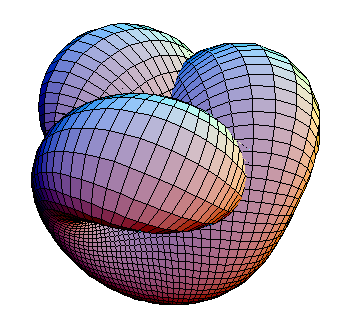
\includegraphics[angle=0,scale=0.7]{imagens/cap2/BoysSurfaceTopView.png} 
\caption{Proje\c{c}\~ao em $\R^3$ do plano projetivo. Figura extra�da de \url{https://commons.wikimedia.org/wiki/File:BoysSurfaceTopView.PNG} } 
\label{fig.BoySurface}
\end{center}
\end{figure}


\begin{figure}[h]
\begin{center} 
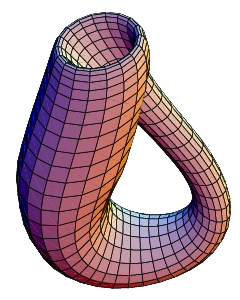
\includegraphics[angle=0,scale=0.7]{imagens/cap2/KleinBottle-01.png} 
\caption{Superf�cie n�o orient�vel chamada de {\bf garrafa de Klein}. Figura extra�da de \url{https://commons.wikimedia.org/wiki/File:KleinBottle-01.png} } 
\label{fig.BoySurface}
\end{center}
\end{figure}

\begin{defi} $($Espa�o Tangente$)$
Sejam $\mathcal{M}$ uma variedade diferenci\'avel de dimens\~ao $n$ e $\varphi : V \rightarrow U \cap \mathcal{M}$ uma parametriza\c c\~ao de $U \cap \mathcal{M}$, onde $\varphi(u) = v$.
Definimos o espa\c co vetorial tangente a $\mathcal{M}$ no ponto $v$ como $T_{v}\mathcal{M} = \{ D\varphi(u) \cdot y \; | \; y \in {\R}^{n}\}$, onde $D\varphi(u)$ � o operador derivada da parametriza��o $\varphi$ no ponto $u \in V$. 
\end{defi}

\begin{teore} $($Variedade Definida Implicitamente$)$ \label{teo_VI}
Sejam $U \subset \R^n$ um aberto e $f : U \rightarrow \R^k$ uma aplica��o de classe $C^r$ $(1 \le r \le \infty)$.
Se $c \in \R^k$ � valor regular de $f$, ou $f^{-1}(c)$ � vazio ou � uma variedade diferenci�vel de dimens�o $n-k$ e de classe $C^r$ em $\R^n$.
Al�m disso, para todo $p \in f^{-1}(c)$, o espa�o tangente em $p$ � o n�cleo de $Df(p): \R^n \rightarrow \R^k$.
\end{teore} 

\begin{teore} $($Vizinhan�a Tubular$)$ \label{teo_VT}
Seja $F : U \rightarrow \R^{n}$ uma aplica\c c\~ao de classe $C^{r}$ no 
aberto $U \subset \R^{m}$ com $m \geq n$ e $1 \le r \le \infty$. 
Se $c \in  \R^{n}$ \'e um valor regular de $F$, ent\~ao existe uma vizinhan\c ca fechada $V_{\mathcal{M}}$ da variedade $\mathcal{M} = F^{-1}(c)$ constitu\'{\i}da de variedades, isto \'e, se $x \in V_{\mathcal{M}}$, ent\~ao $F^{-1}(F(x))$ \'e uma variedade contida em $V_{\mathcal{M}}$.
\end{teore} 

\begin{defi} $($Conjunto de Medida Nula$)$
Uma conjunto $X \subset \R^n$ � um conjunto de medida nula em $\R^n$ se para cada $\epsilon > 0$ dado, � poss�vel obter uma sequ�ncia de hipercubos de dimens�o $n$ abertos $C_1, C_2,\ldots,C_k,\ldots$ em $\R^n$ tais que $X \subset \cup_{k=1}^\infty C_k$ e $\sum_{k=1}^\infty vol(C_k) < \epsilon$.
\end{defi}

\begin{defi} $($Conjunto Denso$)$
Uma conjunto $X \subset \R^n$ � um conjunto denso em $\R^n$ se o complementar $R^n - X$ tem medida nula em $\R^n$.
\end{defi}

\begin{teore} $($Sard$)$ \label{Teo_Sard}
Seja $f : U \subset \R^n \rightarrow \R^k$ uma aplica��o de classe $C^r$ $(r \ge max\{1,n-k+1\})$. 
O conjunto dos valores regulares de $f$ � aberto e denso em $\R^k$.
\end{teore}

\begin{defi} $($Subvariedade Diferenci�vel$)$
Seja $\mathcal{M} \subset \R^m$ uma variedade diferenci�vel de dimens�o $n$ e de classe $C^r$ $(1 \le r \le \infty)$. 
$\mathcal{N} \subset \mathcal{M}$ � uma subvariedade diferenci�vel de dimens�o $k$ de $\mathcal{M}$ e de classe $C^s$ $(1 \le s \le r)$ 
se para todo $x \in \mathcal{N}$ existirem vizinhan�as abertas $U \subset \R^m$ de $x$, 
$V \subset \R^{k-1} \times \R^{+}$ e um difeomorfismo de classe $C^s$ de $\mathcal{N} \cap U$ em $V$.  
\end{defi}

\begin{defi} $($Transversalidade$)$ \label{def_TR}
Sejam $\mathcal{M}$ e $\mathcal{N}$ duas variedades de dimens�o $m$ e $n$ respectivamente em $\R^k$ $(k \ge max\{m , n\})$ e de classe $C^r$ $(1 \le r \le \infty)$. 
Dizemos que $\mathcal{M}$ e $\mathcal{N}$ s�o transversais em um ponto $p \in \mathcal{M} \cap \mathcal{N}$ se $T\mathcal{M}_p + T\mathcal{N}_p = \R^k$.
Se $\mathcal{M} \cap \mathcal{N} = \emptyset$, ent\~ao $\mathcal{M}$ e $\mathcal{N}$ s\~ao transversais por vacuidade.
\end{defi}




\markboth{Variedades}{Variedades Lineares por Partes}
\section{Variedades Lineares por Partes}\label{cap_var_lin_par}

Para maior aprofundamento no tema apresentado nesta e nas pr\'oximas se��es, \'e sugerida a leitura da tese~\cite{Cas92}, do livro~\cite{AlGe90}, do artigo~\cite{Cas06} e do curso no proceedings~\cite{Eaves76}. 

\begin{defi} $($Espa�o Afim$)$
Dados os pontos $v_{0},v_{1},\ldots,v_{k} \in \R^{n}$, chama-se o conjunto 
$aff(v_{0},\ldots,v_{k}) =$ 
$\{ v \in  \R^{n} \; |$ $ \sum_{i=0}^{k} \lambda_{i} v_{i} = v$ e 
$\sum_{i=0}^{k} \lambda_{i} = 1\}$ de conjunto afim gerado pelos pontos
$v_{0},\ldots,v_{k}$.  
\end{defi}

\begin{defi} $($Dimens�o$)$
Chama-se de dimens\~ao de $aff(v_{0},\ldots,v_{k})$ 
e denota-se por $dim(aff(v_{0},\ldots,v_{k}))$ o maior n\'umero de vetores 
linearmente independentes entre os do conjunto
$\{v_{1}-v_{0},\ldots,v_{k}-v_{0}\}$.
\end{defi}

\begin{defi} $($C�lula Convexa Afim$)$
Chama-se de c\'elula convexa afim, gerada pelos
pontos $v_{0},v_{1},\ldots,v_{k}$, o conjunto 
$\sigma = [v_{0},\ldots,v_{k}]$ $ = \{ v \in  \R^{n} \; | \;
\sum_{i=0}^{k} \lambda_{i} v_{i} = v, \sum_{i=0}^{k} \lambda_{i} = 1$
e $\lambda_{i} \geq 0 \}$. Definimos a dimens\~ao de $\sigma$ por
$dim(\sigma) =$ $dim(aff(v_{0},\ldots,$ $v_{n}))$. 
Uma c�lula convexa afim $\sigma$ de dimens�o $k$ � denominada $k$-c�lula.
\end{defi}

\begin{figure}[h]
\begin{center}
\begin{tabular}{ccc}
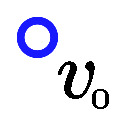
\includegraphics[angle=0,scale=0.45]{imagens/cap2/fig6-0.eps} & \hspace{0.5cm} 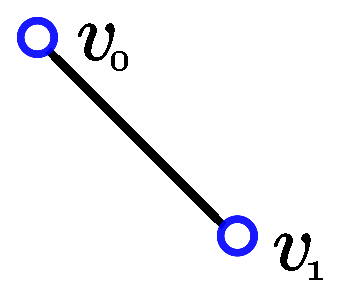
\includegraphics[angle=0,scale=0.45]{imagens/cap2/fig6-1.eps} & \hspace{0.5cm}
 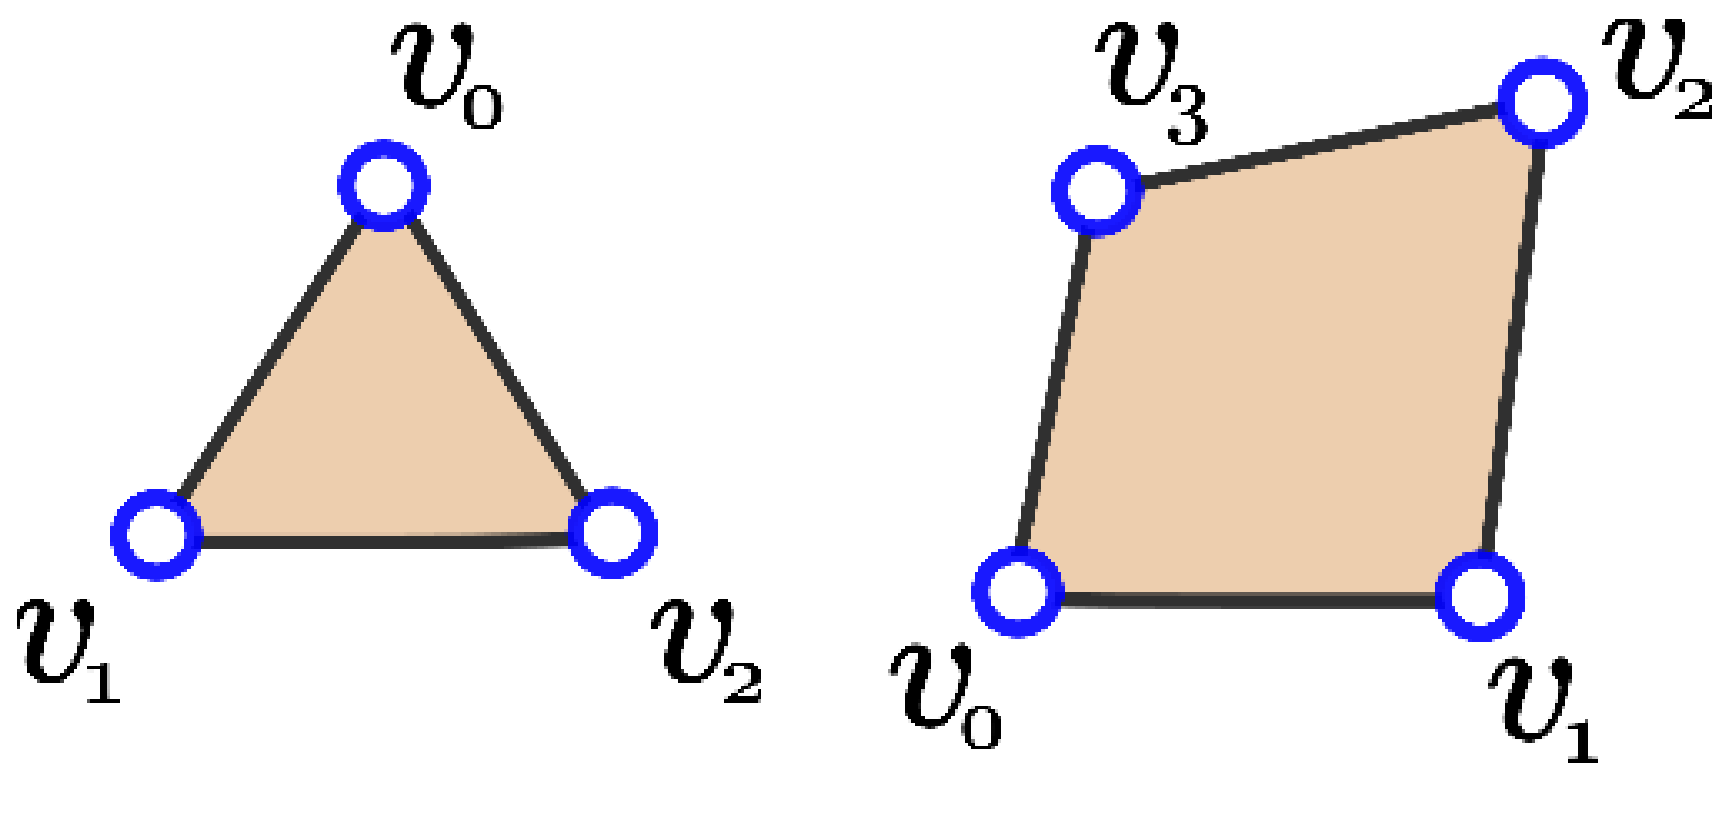
\includegraphics[angle=0,scale=0.2]{imagens/cap2/fig6-2.eps}\\
 0-c�lula & \hspace{0.5cm} 1-c�lula & \hspace{0.5cm} 2-c�lula\\
 \end{tabular} 
 \begin{tabular}{c}
 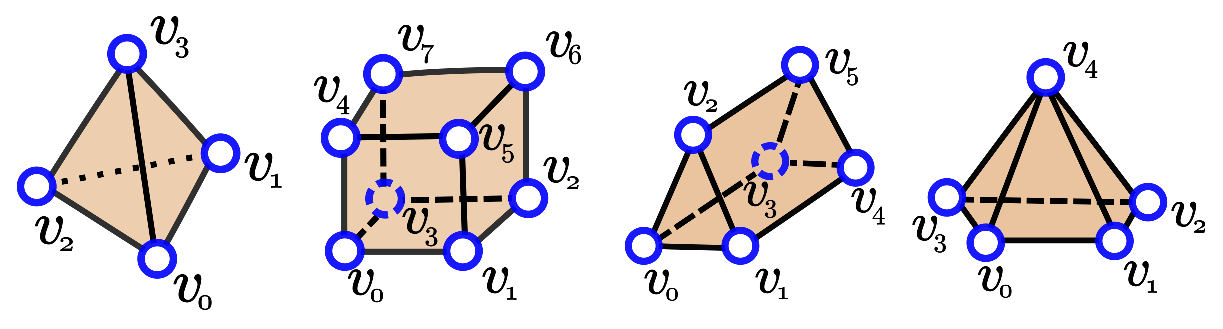
\includegraphics[angle=0,scale=0.65]{imagens/cap2/fig6-3.eps} \\
3-c�lula \\
\end{tabular}
\end{center}
\caption{Exemplos de 0-c�lula, 1-c�lula, 2-c�lulas e 3-c�lulas.}
\end{figure}


\begin{defi} $($Bordo de uma C�lula Convexa Afim$)$
O bordo de uma c\'elula convexa afim $\sigma$, denotada por $\partial(\sigma)$,
� o conjunto de sub-c�lulas satisfazendo:
\begin{enumerate}
\item Se $\sigma' \in \partial(\sigma)$, ent�o $\sigma'$ � gerada por um subconjunto de v�rtices de $\sigma$;
\item Para qualquer $p \in \sigma' \in \partial(\sigma)$, n�o existe uma bola contendo $p$ em $aff(\sigma)$ inteiramente contida em $\sigma'$;
\item Se $\sigma'_1, \sigma'_2 \in \partial(\sigma)$ e tem a mesma dimens�o ent�o  $\sigma'_1 \nsubseteq \sigma'_2$ e $\sigma'_2 \nsubseteq \sigma'_1$.
\end{enumerate}
\end{defi}

\begin{defi} $($Face de uma C�lula Convexa Afim$)$
Sejam uma c�lula convexa afim $\sigma = [v_{0},\ldots,v_{m}]$ de dimens�o $n$ e
$\tau = [\omega_{0},\ldots,\omega_{l}]$ uma c�lula convexa afim de dimens�o $k$,
com $\{\omega_{0},\ldots,\omega_{l}\} \subset \{v_{0},\ldots,v_{m}\}$, 
ent�o $\tau$ � uma face de $\sigma$ se:
\begin{enumerate}
\item $\tau \subset \partial(\sigma)$; 
\item Se existe alguma sub-c�lula $\eta$ com $aff(\tau) = aff(\eta)$, ent�o $\eta \subset \tau$.
\end{enumerate}
\end{defi}

\begin{defi} $($Decomposi��o Celular$)$
Uma cole\c c\~ao $\mathcal{C}$ de c\'elulas convexas afins 
\'e dita decomposi\c c\~ao celular de um conjunto $S \subset  \R^{n}$ se:
\begin{enumerate}
\item $S = \bigcup_{\sigma \in \mathcal{C}}\ \sigma$;
\item Se $\sigma_{1},\sigma_{2} \in \mathcal{C}$, ent\~ao $\sigma_{1} \cap \sigma_{2} = 
         \emptyset$ ou $\sigma_{1} \cap \sigma_{2} \in \mathcal{C}$;
\item Todo subconjunto compacto de $S$ intersecta um n\'umero finito de
      c\'elulas de $\mathcal{C}$. 
\end{enumerate}
\end{defi}

\begin{defi} $($Complexo Celular$)$
Um complexo celular $\mathcal{C}$ � um conjunto finito de c�lulas convexas afins que satisfazem: 
\begin{enumerate}
\item Se $\sigma \in \mathcal{C}$ e $\tau$ face de $\sigma$ ent�o $\tau \in \mathcal{C}$;
\item Se $\sigma_{1},\sigma_{2} \in \mathcal{C}$, ent\~ao $\sigma_{1} \cap \sigma_{2} = \emptyset$ ou $\sigma_{1} \cap \sigma_{2}$ � uma face comum de $\sigma_1$ e $\sigma_2$.
\end{enumerate}
\label{complexocelular}
\end{defi}

A intersec��o entre duas c�lulas quaisquer de um complexo celular se d� por uma face comum a ambas.  A Figura \ref{fig.celula}-(a) apresenta um exemplo de um complexo celular bidimensional, enquanto a figura \ref{fig.celula}-(b)) apresenta um contra-exemplo de complexo celular. 


\begin{figure}[h]
\begin{center} 
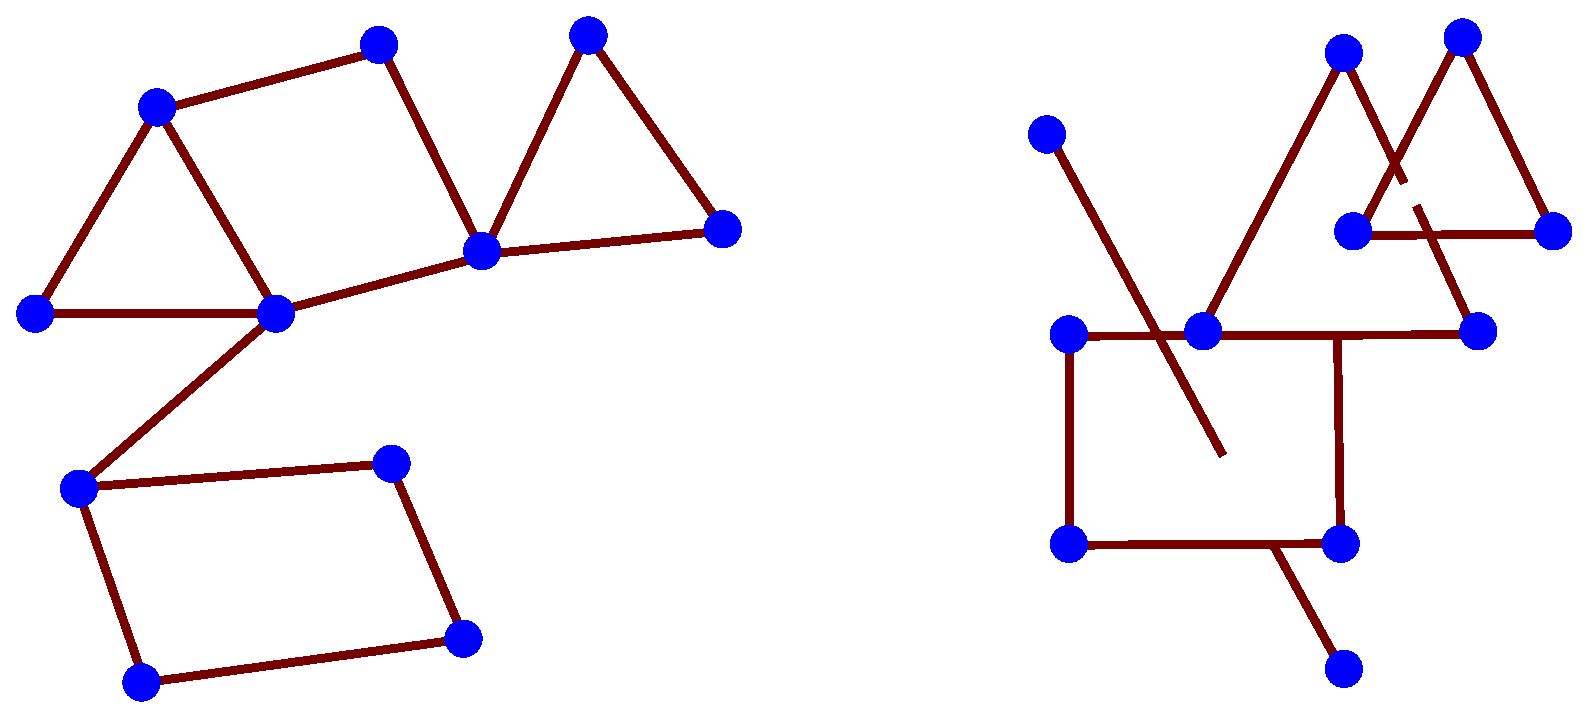
\includegraphics[angle=0,scale=0.3]{imagens/cap2/fig1.eps} \\
(a) \hspace{5.0cm} (b)\\
\caption{(a) Exemplo de complexo celular e (b) contra-exemplo de complexo celular.} 
\label{fig.celula}
\end{center}
\end{figure}


\begin{defi} $($Simplexo$)$
Uma c\'elula convexa afim 
$\sigma = [v_{0},\ldots,v_{k}]$ de $\R^{n}$ \'e chamada de simplexo, se 
$dim(\sigma) = k$, isto \'e, um simplexo $k$-dimensional \'e uma c\'elula 
convexa afim de dimens\~ao $k$ gerada por $k+1$ pontos. 
Um simplexo de dimens�o 0 � denominado v�rtice e um simplexo de dimens�o 1 � denominado aresta.
\end{defi}

\begin{defi} $($Triangula��o$)$
Uma decomposi\c c\~ao celular $\mathcal{C}$ de 
$S \subset \R^{n}$ \'e chamada de triangula\c c\~ao de $S$, se
todas as c\'elulas de $\mathcal{C}$ s\~ao simplexos. 
\end{defi}

\begin{defi} $($Complexo Simplicial$)$
Um complexo simplicial � um complexo celular $\mathcal{C}$ onde todas as c�lula de $\mathcal{C}$ s�o simplexos.
\end{defi}

\begin{defi} $($Propriedades de Simplexos$)$
Dado um simplexo 
$\sigma = [v_{0}, \ldots, v_{k}]$ de $\R^{n}$, define-se : 
\begin{enumerate} 
\item A fronteira de $\sigma$, $\partial \sigma$, como a uni\~ao de todas as
      faces de dimens\~ao $k-1$ de $\sigma$; 
\item O baricentro de $\sigma$, $b(\sigma) = \frac{1}{k+1} \sum_{i=0}^{k}
      v_{i}$; 
\item O di\^ametro de $\sigma$, $\rho(\sigma) = max \{\parallel v_{i}-v_{j} 
\parallel; i, j = 0, \ldots, k\}$;
\item O raio de $\sigma$, $r(\sigma) = min \{\parallel v-b(\sigma) \parallel \; | \;
       v \in \partial(\sigma)\}$;
\item A robustez de $\sigma$, $\theta(\sigma) = r(\sigma)/\rho(\sigma)$.
\end{enumerate} 
\end{defi}

\begin{defi} $($Propriedades de Triangula��o$)$
Se $T$ \'e uma triangula\c c\~ao de 
$S \subset \R^{n}$, define-se: 
\begin{enumerate} 
\item O di\^ametro de $T$, $\rho(T) = sup \{ \rho(\sigma) \; | \; \sigma \in T$ 
      com $dim(\sigma) > 0 \}$;
\item A robustez de $T$, $\theta(T) = inf \{ \theta(\sigma) \; | \; \sigma \in T$ 
      com $dim(\sigma) > 0 \}$.
\end{enumerate} 
\end{defi}

\begin{defi} $($C�lulas Adjacentes$)$
Uma c�lula $\sigma_1$ � dita adjacente a outra c�lula $\sigma_2$ se $\sigma_1 \cap \sigma_2$ � uma face comum de $\sigma_1$ e $\sigma_2$.
\end{defi}

A Figura \ref{fig.adjacente} apresenta dois exemplos de adjac�ncia entre c�lulas, um de c�lulas bidimensionais e outro de c�lulas tridimensionais.

\begin{figure}[h]
\begin{center} 
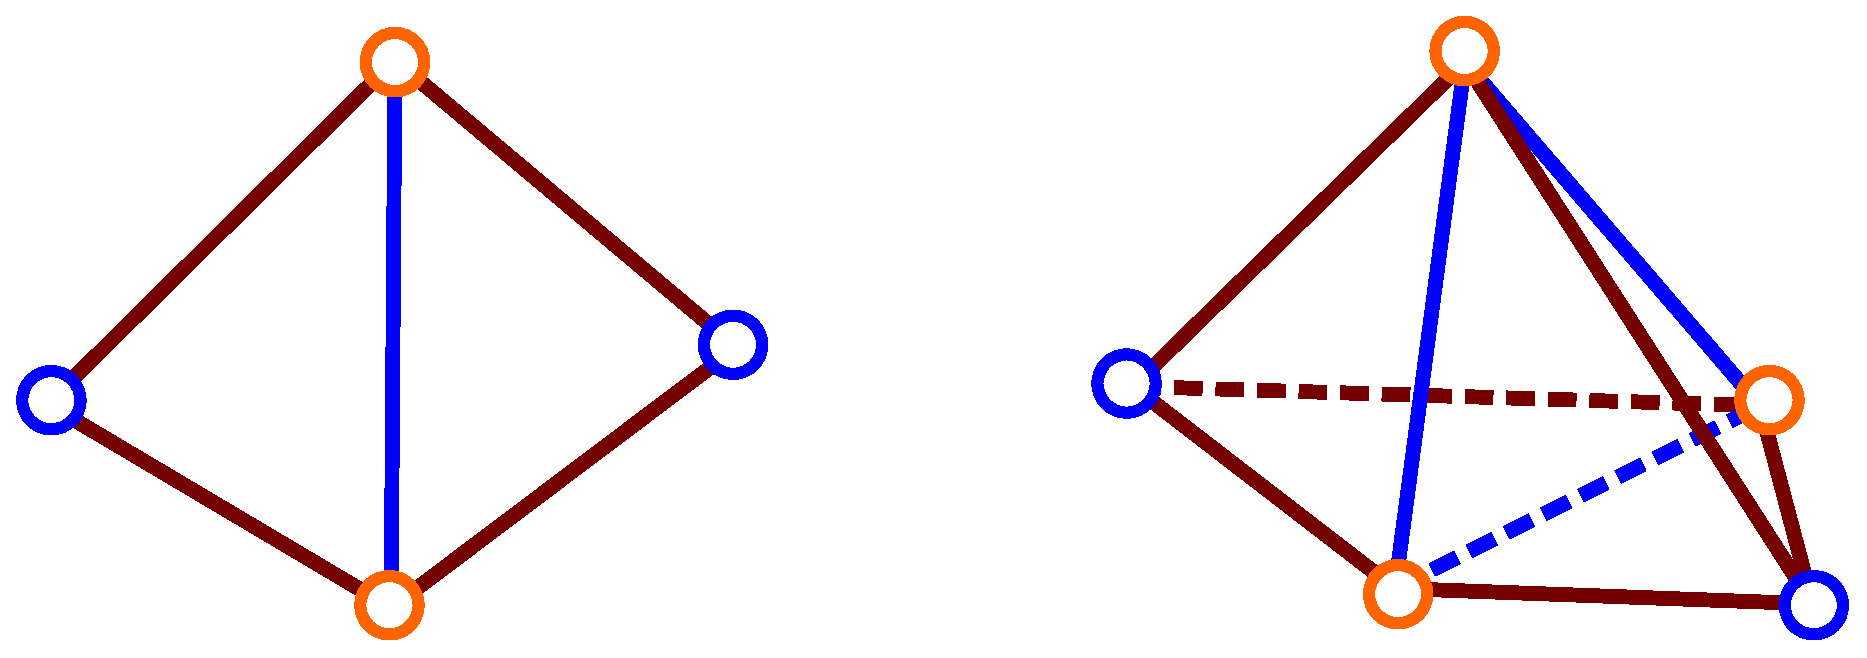
\includegraphics[angle=0,scale=0.3]{imagens/cap2/fig2.eps} \\
(a)Adjac�ncia entre 2-c�lulas \hspace{1.cm} (b) Adjac�ncia entre 3-c�lulas
\caption{Adjac�ncias entre 2-c�lulas (por uma aresta) e 3-c�lulas (por uma face).} 
\label{fig.adjacente}
\end{center}
\end{figure}

\begin{defi} $($V�rtices Vizinhos$)$
Um v�rtice � dito vizinho a outro se existe uma aresta que cont�m os dois.
\end{defi}

\begin{defi} $($C�lulas Incidentes$)$
Dada uma c�lula $\sigma$ de dimens�o $p$ e $\tau$ uma c�lula de dimens�o $k$, onde $p > k$, estas c�lulas s�o ditas incidentes se $\tau$ � uma face de $\sigma$. 
\end{defi}

\begin{defi} $($Orienta��o de uma C�lula$)$
Seja $\mathcal{C}$ um complexo celular de dimens�o $p$, onde $p$ � a maior dimens�o de todas as c�lulas. A orienta��o de duas c�lulas adjacentes $\sigma$ e $\tau$ de dimens�o $p$ de $\mathcal{C}$ � coerente se face de dimens�o $p-1$ que compartilham tem orienta��o oposta em cada uma das c�lulas. O complexo celular $\mathcal{C}$ � orient�vel se uma orienta��o coerente pode ser escolhida para todas as suas c�lulas.
\end{defi}


\begin{figure}[h]
\begin{center} 
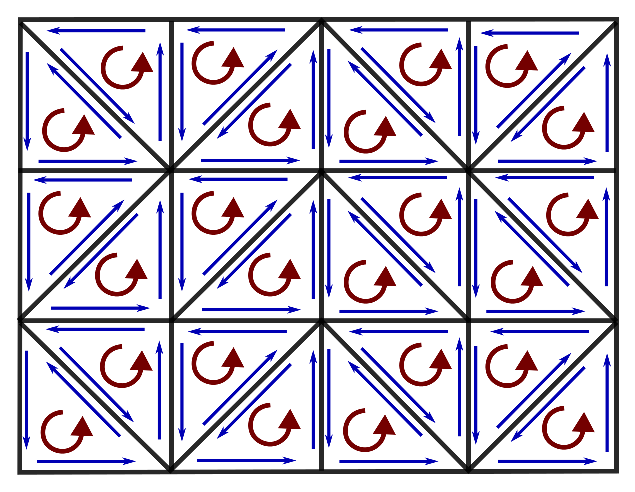
\includegraphics[angle=0,scale=0.7]{imagens/cap2/fig3.eps}
\caption{Complexo celular bidimensional orientado em sentido anti-hor�rio.} 
\label{fig.orientacao}
\end{center}
\end{figure}


\begin{defi} $($Estrela de uma C�lula$)$
A estrela de uma c�lula $\sigma$ de um complexo celular $\mathcal{C}$, denominada por $S(\sigma)$ � o conjunto de todas as c�lulas de $\mathcal{C}$ que cont�m $\sigma$, isto �, $S(\sigma) = \{ \tau \in \mathcal{C} \; | \; \sigma \subseteq \tau \}$.
\end{defi}

\begin{defi} $($Elo de uma C�lula$)$
O elo de uma c�lula $\sigma \subset \mathcal{C}$ � o conjunto $L(\sigma) = \{ \tau \in \overline{S(\sigma)} \; | \; \tau \cap \sigma = \emptyset \}$, onde $\overline{S(\sigma)}$ � o fecho da estrela de $\sigma$.
\end{defi}

Um exemplo de estrela e de elo de um v�rtice central � mostrado na Figura \ref{fig.elo}(b). 

\begin{figure}[h]
\begin{center} 
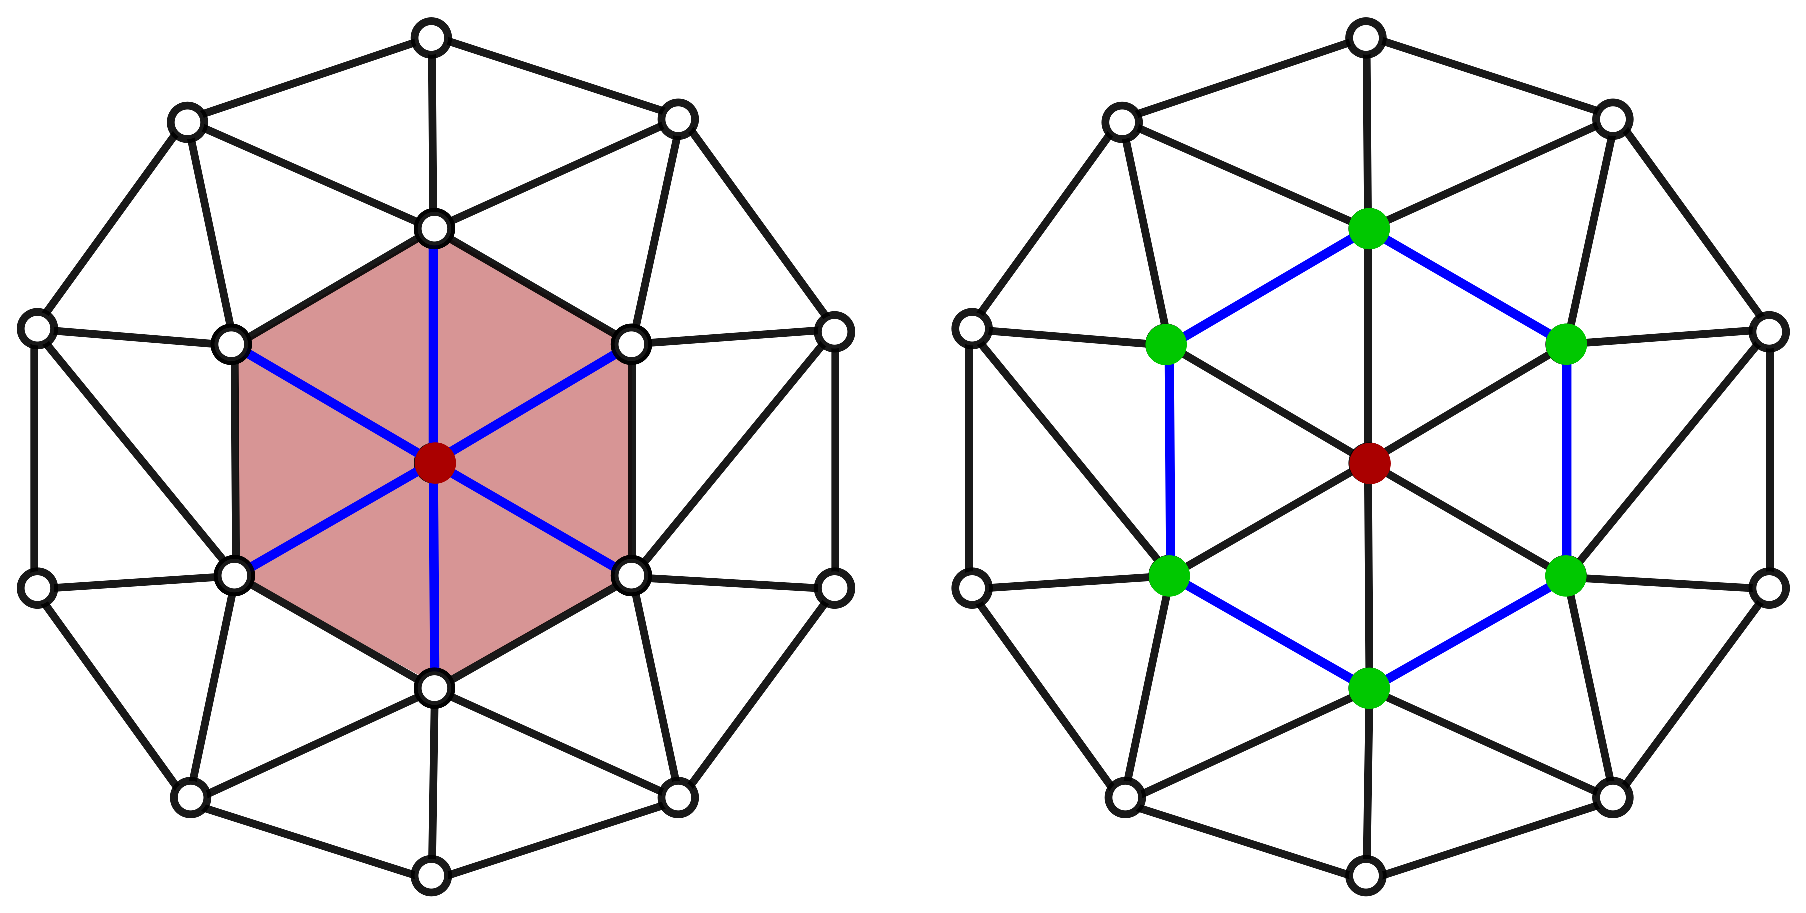
\includegraphics[angle=0,scale=0.35]{imagens/cap2/fig4.eps}\\
(a) Estrela do v�rtice central \hspace{1.0cm} (b) Elo do v�rtice central\\
\caption{Representa��es de uma estrela e um elo de um v�rtice.} 
\label{fig.elo}
\end{center}
\end{figure}


\begin{defi} $($Variedade Linear por Partes$)$
Um complexo celular $\mathcal{C}$ de dimens�o $n$ � dito uma variedade linear por partes de dimens�o $n$ se para todo $\sigma \in \mathcal{C}$, ou $L(\sigma)$ � homeomorfo a uma esfera de dimens�o $n-1$, ou � homeomorfo a um disco de dimens�o $n-1$. 
Caso $L(\sigma)$ seja homeomorfo a um disco de dimens�o $n-1$, $\sigma$ pertence ao bordo de $\mathcal{C}$. 
\end{defi}


A figura \ref{fig.varLinPartes}-(a) d� um exemple de um v�rtice de interior, enquanto a figura \ref{fig.varLinPartes}-(b) exemplifica um v�rtice de bordo de uma variedade linear por partes de dimens�o 2. 
J� a figura \ref{fig.varLinPartes}-(c) exibe uma n�o-variedade. 

\begin{figure}[h]
\begin{center} 
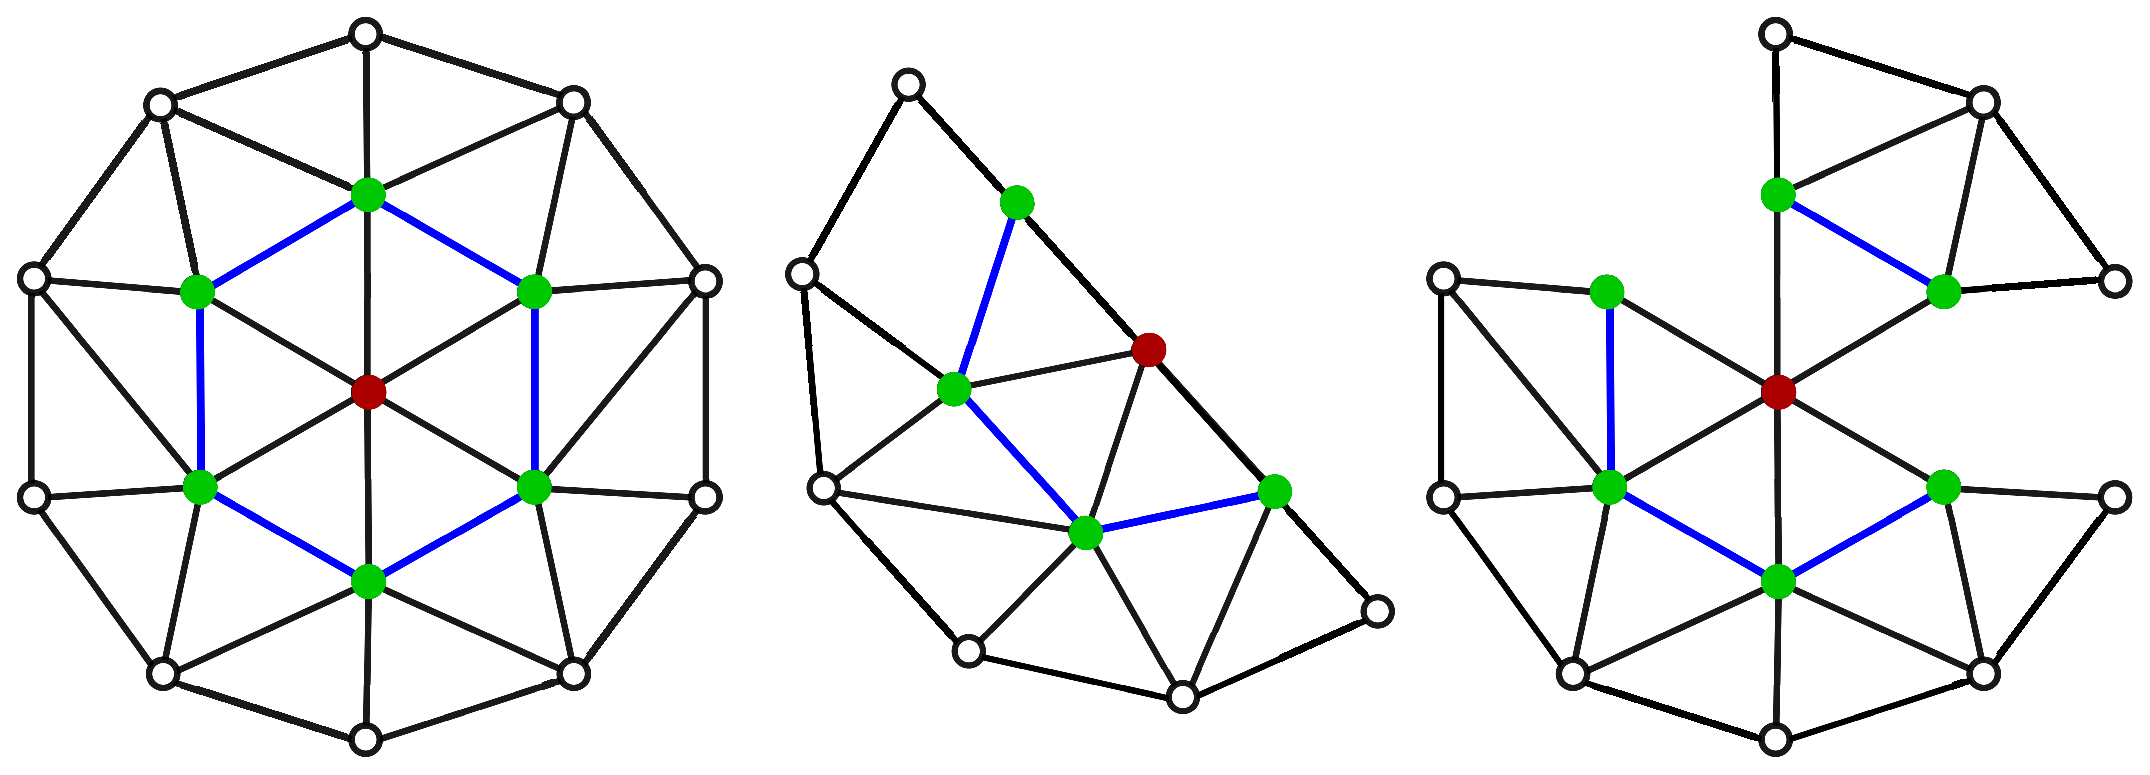
\includegraphics[angle=0,scale=0.35]{imagens/cap2/fig5.eps}\\
(a) Ponto de interior \hspace{0.8cm} (b) Ponto de Bordo \hspace{0.8cm} (c) N�o-variedade
\caption{Exemplos de variedades (a) e (b) e de n�o-variedade (c).} 
\label{fig.varLinPartes}
\end{center}
\end{figure}

\begin{defi} $($Variedade Triangulada$)$
Uma variedade triangulada $\mathcal{C}$ � uma variedade linear por partes onde todas suas c�lulas s�o simplexos.
\end{defi}




\markboth{Variedades}{Formas de Representa��o de Variedades}
\section{Formas de Representa��o de Variedades}\label{var_formas}

As formas de representa��o mais comuns de variedades s�o como gr�fico de uma fun��o, a imagem de uma fun��o e como a imagem inversa de uma fun��o.
Estas formas de reapresenta��o ser�o definidas e exemplificadas nas pr�ximas subse��es.


\markboth{Variedades}{Variedades como Gr�fico de Fun��es}
\subsection{Variedades como Gr�fico de Fun��es}\label{var_grafico}


Seja $F: U \subset \R^n \rightarrow \R$ de classe $C^r$. O conjunto
$\mathcal{M} = \{ \; (x,F(x)) \; | \; x \in U \; \}$ � uma variedade de dimens�o $n$ em $\R^{n+1}$ de classe $C^r$.
Neste caso $\mathcal{M}$ � o gr�fico da fun��o $F$.

Os casos mais simples s\~ao:
\begin{itemize}
 \item Para $n=1$ o gr�fico de $F$ \'e uma curva em $\R^2$;
 \item Para $n=2$ o gr�fico de $F$ \'e uma superf\'icie em $\R^3$.
\end{itemize}

\noindent {\bf Exemplo 1:} Como exemplo de curva em $\R^2$, apresentamos o c�digo \ref{senocoseno} em Matlab/Octave com o gr�fico das fun��es cosseno e seno. A figura \ref{fig.CosSin} apresenta o resultado da execu��o deste c�digo. 

\begin{Codigo}[htpb]
\noindent\rule{13cm}{1.pt}
\begin{verbatim}
x  = linspace(0,2*pi,30);              % gerando os pontos do dom�nio
y1 = cos(x);                           % gerando a fun��o cosseno 
y2 = sin(x);                           % gerando a fun��o seno 
hold on
plot(x,y1,'r-s');                      % plotando o gr�fico do cosseno
plot(x,y2,'g-*');                      % plotando o gr�fico do seno
grid                                   % gerando um grid
xlabel('eixo x');                      % legenda no eixo horizontal
ylabel('eixo y');                      % legenda no eixo vertical
title('Grafico do seno e do cosseno'); % t�tulo do gr�fico 
legend('sen(x)','cos(x)');             % legenda
hold off
\end{verbatim}
\vspace{-0.5cm}
\caption{C�digo utilizado para gerar a figura \ref{fig.CosSin} } 
\noindent\rule{13cm}{1.pt}
\label{senocoseno}
\end{Codigo}

\begin{figure}[htpb]
\begin{center} 
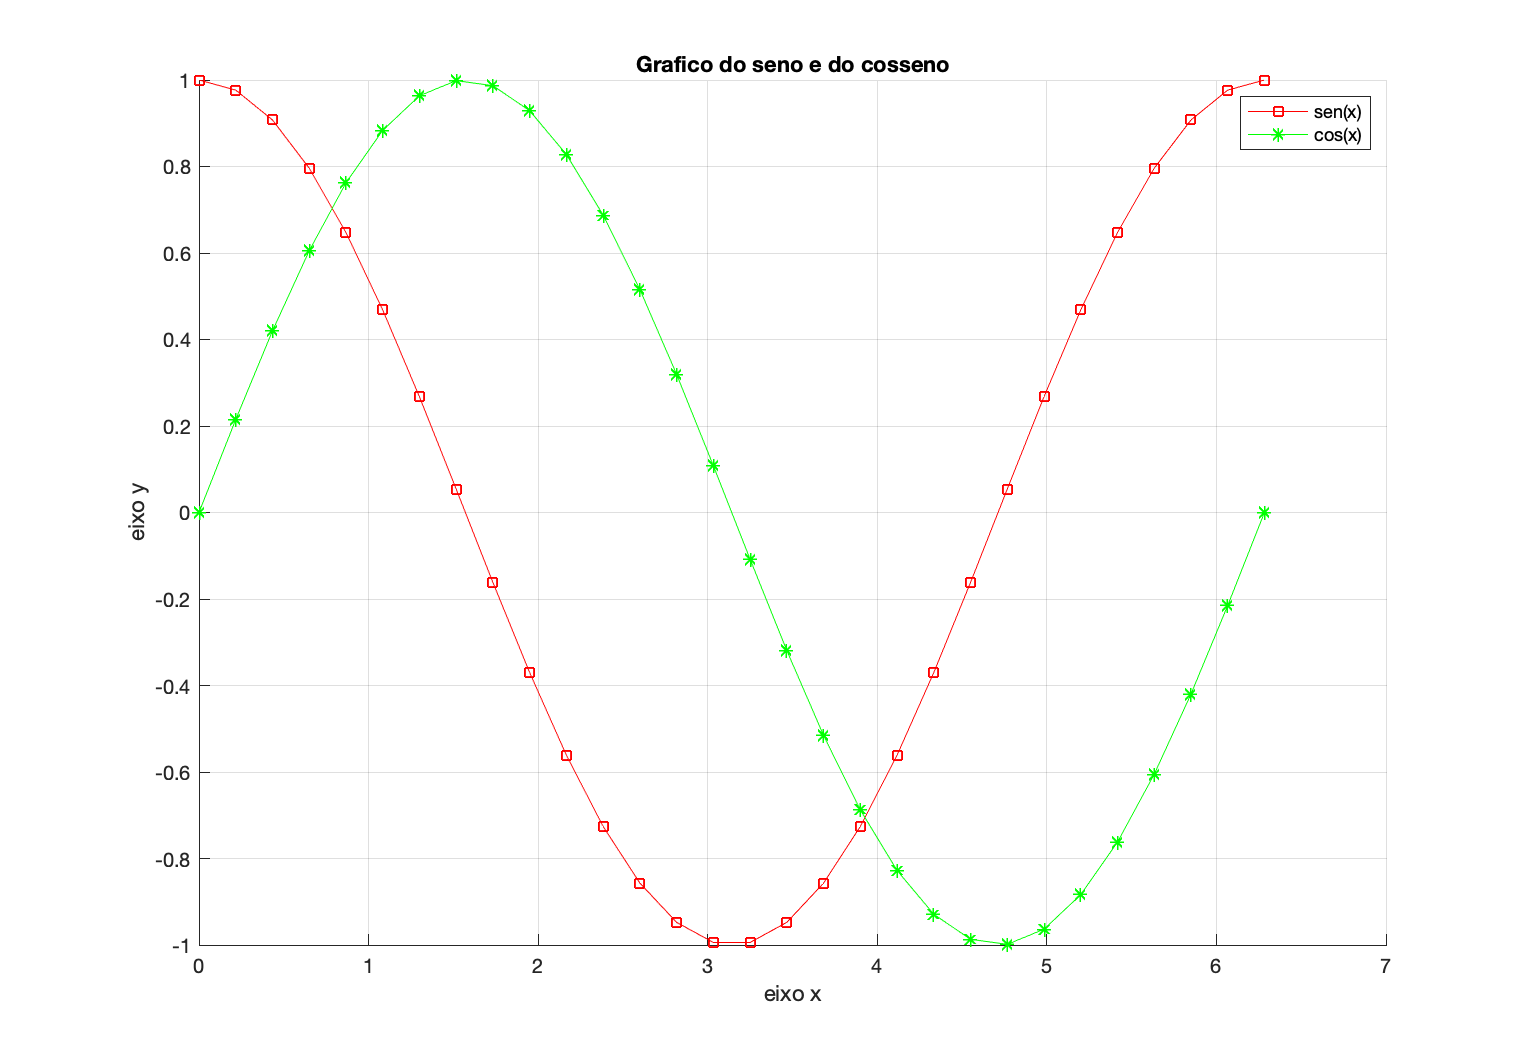
\includegraphics[angle=0,scale=0.17]{imagens/cap2/CosSin.png} 
\vspace{-0.5cm}
\caption{Curvas em $\R^2$ geradas como gr�fico das fun��es cosseno e seno.} 
\label{fig.CosSin}
\end{center}
\end{figure}

\noindent {\bf Exemplo 2:} Como exemplo de superf�cie em $\R^3$, apresentamos o gr�fico da fun��o $z=F(x,y)=\frac{sen(\sqrt{x^2+y^2}+0.1)}{\sqrt{x^2+y^2}+0.1}$. A figura \ref{fig.3d_1} apresenta o resultado da execu��o do c�digo \ref{fig3d} feito em Matlab/Octave.

\begin{Codigo}[htpb]
\noindent\rule{13cm}{1.pt}
\begin{verbatim}
px = py = linspace (-10, 10, 50)';     % gerando os pontos do dom�nio
[x, y] = meshgrid (px, py);            % criando a malha 
r = sqrt(x.^2 + y.^2) + 0.1;           % r � vari�vel auxiliar
z = sin(r) ./ r;                       % fun��o z=F(x,y) 
surf (x, y, z);                        % plotando a superf�cie
xlabel('eixo x');                      % legenda no eixo x
ylabel('eixo y');                      % legenda no eixo y
zlabel('F(x,y)');                      % legenda no eixo z
title('Exemplo de Superficie');        % t�tulo do gr�fico 
legend('Superficie z=F(x,y)');         % legenda
\end{verbatim}
\vspace{-0.5cm}
\caption{C�digo utilizado para gerar a figura \ref{fig.3d_1} } 
\noindent\rule{13cm}{1.pt}
\label{fig3d}
\end{Codigo}

\begin{figure}[htpb]
\begin{center} 
\includegraphics*[angle=0,scale=0.4]{imagens/cap2/superficie.png} 
\vspace{-0.5cm}
\caption{Superf�cie dada pela fun��o $F(x,y)=\frac{sen(\sqrt{x^2+y^2}+0.1)}{\sqrt{x^2+y^2}+0.1}$} 
\label{fig.3d_1}
\end{center}
\end{figure}


Substituindo o comando {\it surf} pelo comando {\it mesh} obtemos o gr�fico $z=F(x,y)$ apenas nos pontos do {\it grid} do dom�nio. A figura \ref{fig.3d_2} apresenta o resultado usando mesh (ver c�digo  \ref{mesh}).


\begin{Codigo}[htpb]
\noindent\rule{13cm}{1.pt}
\begin{verbatim}
px = py = linspace (-10, 10, 50)';     % gerando os pontos do dom�nio
[x, y] = meshgrid (px, py);            % criando a malha 
r = sqrt(x.^2 + y.^2) + 0.1;           % r � vari�vel auxiliar
z = sin(r) ./ r;                       % fun��o z=F(x,y) 
mesh (x, y, z);                        % plotando a superf�cie
xlabel('eixo x');                      % legenda no eixo x
ylabel('eixo y');                      % legenda no eixo y
zlabel('F(x,y)');                      % legenda no eixo z
title('Exemplo de Superficie');        % t�tulo do gr�fico 
legend('Superficie z=F(x,y)');         % legenda
\end{verbatim}
\vspace{-0.5cm}
\caption{C�digo utilizado para gerar a figura \ref{fig.3d_2} } 
\noindent\rule{13cm}{1.pt}
\label{mesh}
\end{Codigo}

\begin{figure}[htpb]
\begin{center} 
\includegraphics*[angle=0,scale=0.4]{imagens/cap2/malha.png} 
\vspace{-0.5cm}
\caption{Superf�cie gerada pela fun��o $F(x,y)=\frac{sen(\sqrt{x^2+y^2}+0.1)}{\sqrt{x^2+y^2}+0.1}$ nos pontos do {\it grid}} 
\label{fig.3d_2}
\end{center}
\end{figure}

\markboth{Variedades}{Variedades Parametrizadas}
\subsection{Variedades Parametrizadas}\label{var_param}

Seja $F: U \subset \R^k \rightarrow \R^n$, $ n \geq k$, de classe $C^r$. O conjunto
$\mathcal{M} = \{ \; F(x) \; | \; x \in U \; \}$ � uma variedade de dimens�o $k$ em $\R^{n}$ de classe $C^r$.
Neste caso $\mathcal{M}$ � a imagem da fun��o $F$, e $F$ � denominada parametriza��o de $\mathcal{M}$.

As parametriza��es mais comuns s�o tratadas nos curso de c\'alculo e geometria diferencial:
\begin{itemize}
 \item Para $n=2$ e $k=1$, $F(x)$ \'e uma curva em $\R^2$;
 \item Para $n=3$ e $k=1$, $F(x)$ \'e uma curva em $\R^3$;
 \item Para $n=3$ e $k=2$, $F(x)$ \'e uma superf\'icie em $\R^3$.
\end{itemize}

\noindent {\bf Exemplo 1:} Uma exemplo de curva parametrizada em $\R^2$ � apresentada  em \ref{fig.pplanacurva} e foi gerada pelo c�digo \ref{pplanacurva} em Matlab/Octave.

\begin{Codigo}[htpb]
\noindent\rule{13cm}{1.pt}
\begin{verbatim}
t = linspace(-2,2,80);                   % intervalo do par�metro t
f = @(t) t.^2+1.0;                       % gerando a fun��o f
g = @(t) t.*cos(t);                      % gerando a fun��o g 
plot(f(t), g(t));                        % plotando 
grid                                     % gerando um grid
xlabel('f(t)');                          % legenda no eixo horizontal
ylabel('g(t)');                          % legenda no eixo vertical
title('Exemplo de curva Parametrizada'); % t�tulo do gr�fico 
legend('Curva F(t)=(f(t),g(t))');        % legenda
\end{verbatim}
\vspace{-0.5cm}
\caption{C�digo utilizado para gerar a figura \ref{fig.pplanacurva} } 
\noindent\rule{13cm}{1.pt}
\label{pplanacurva}
\end{Codigo}


\begin{figure}[htpb]
\begin{center} 
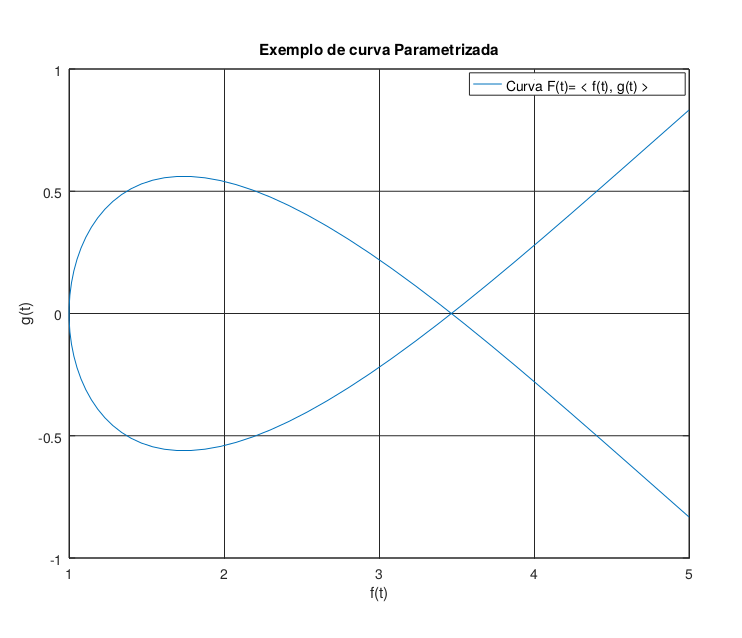
\includegraphics[angle=0,scale=0.4]{imagens/cap2/pplanacurva.png}
\vspace{-0.5cm}
\caption{Curva $F(t) = (t^2+1, t\ cos(t))$, $t=[-2:2]$} 
\label{fig.pplanacurva}
\end{center}
\end{figure}

\noindent {\bf Exemplo 2:} Como exemplo de curva parametrizada em $\R^3$, apresentamos o c�digo em Matlab/Octave \ref{pespcurva}. A figura \ref{fig.pespcurva} apresenta o resultado da execu��o deste c�digo.

\begin{Codigo}[htpb]
\noindent\rule{13cm}{1.pt}
\begin{verbatim}
t = linspace(0,20,100);                     % intervalo do par�metro t
plot3(sin(t),cos(t),t);                     % plotando 
grid                                        % gerando um grid
xlabel('eixo x')                            % legenda no eixo x
ylabel('eixo y')                            % legenda no eixo y
zlabel('eixo z')                            % legenda no eixo z
axis square
title('Exemplo de curva Parametrizada');         % t�tulo do gr�fico 
legend('Curva F(t)=(sin(t),cos(t),t),t=[0,20]'); % legenda
\end{verbatim}
\vspace{-0.5cm}
\caption{C�digo utilizado para gerar a figura \ref{fig.pespcurva} } 
\noindent\rule{13cm}{1.pt}
\label{pespcurva}
\end{Codigo}

\begin{figure}[htpb]
\begin{center} 
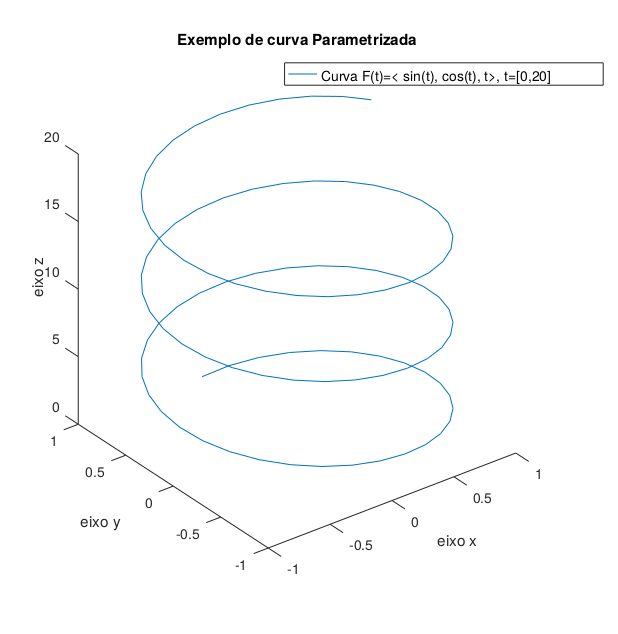
\includegraphics[angle=0,scale=0.4]{imagens/cap2/pespcurva.png} 
\caption{Curva em $\R^3$ da fun��o $F(t)= (sin(t), cos(t), t)$ , $t=[0,20]$ } 
\label{fig.pespcurva}
\end{center}
\end{figure}

\noindent {\bf Exemplo 3:}  Como exemplo de superf�cie parametrizada em $\R^3$, apresentamos o c�digo em Matlab/Octave \ref{pespsurf}. A figura \ref{fig.pespsurf} apresenta o resultado da execu��o deste c�digo.

\begin{Codigo}[htpb]
\noindent\rule{13cm}{1.pt}
\begin{verbatim}
t = linspace(0,10,40);                      % intervalo do par�metro t 
u = linspace(-2,2,40);                      % intervalo do par�metro u
[t,u] = meshgrid(t,u);                      % gerando a malha
x = 2.*t;                                   % f(t,u)
y = 3*u.*cos(t);                            % g(t,u)
z = u.*sin(t);                              % h(t,u)
surf(x,y,z);                                % plotando
xlabel('eixo x')                            % legenda no eixo x
ylabel('eixo y')                            % legenda no eixo y
zlabel('eixo z')                            % legenda no eixo z
axis square
title('Exemplo de Superf�cie Parametrizada');  % t�tulo do gr�fico 
legend('Superficie F(t,u)');                   % legenda
\end{verbatim}
\vspace{-0.5cm}
\caption{C�digo utilizado para gerar a figura \ref{fig.pespsurf} } 
\noindent\rule{13cm}{1.pt}
\label{pespsurf}
\end{Codigo}

\begin{figure}[htpb]
\begin{center} 
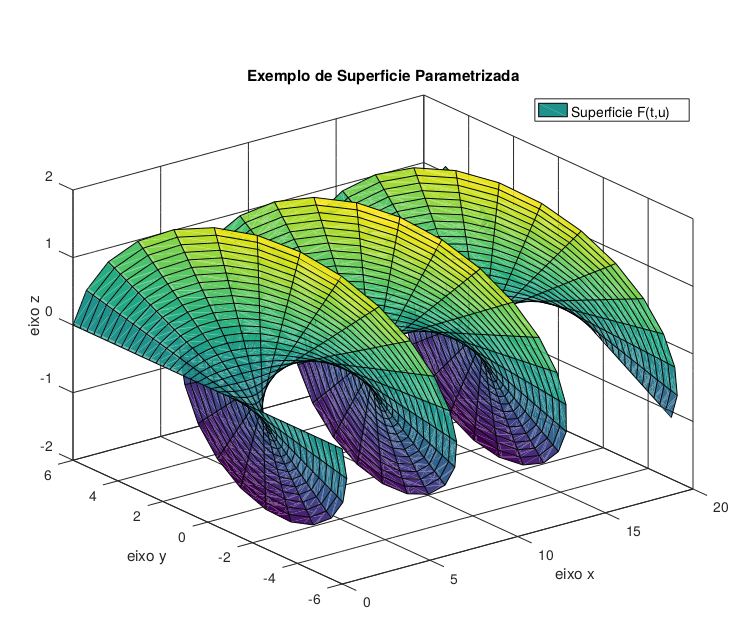
\includegraphics[angle=0,scale=0.4]{imagens/cap2/pespsurf.png} 
\caption{Superf�cie $F(t,u) = (f(t,u), g(t,u), h(t,u))$, $t=[0,10]$, $u=[-2,2]$, $f(t,u)=2\ t$, $g(t,u)=3\ u\ cos(t)$, $h(t,u)=u\ sen(t)$.} 
\label{fig.pespsurf}
\end{center}
\end{figure}

Substituindo o comando {\it surf} pelo comando {\it mesh} (ver c�digo \ref{pespmesh}) obtemos o gr�fico anterior apenas nos pontos do {\it grid} do dom�nio (ver  figura \ref{fig.pespmesh}). 

\begin{Codigo}[htpb]
\noindent\rule{13cm}{1.pt}
\begin{verbatim}
t = linspace(0,10,40);                     % intervalo do par�metro t 
u = linspace(-2,2,40);                     % intervalo do par�metro u
[t,u] = meshgrid(t,u);                     % gerando a malha
x = 2.*t;                                  % f(t,u)
y = 3*u.*cos(t);                           % g(t,u)
z = u.*sin(t);                             % h(t,u)
mesh(x,y,z);                               % plotando
xlabel('eixo x')                           % legenda no eixo x
ylabel('eixo y')                           % legenda no eixo y
zlabel('eixo z')                           % legenda no eixo z
axis square
title('Exemplo de Superf�cie Parametrizada');  % t�tulo do gr�fico 
legend('Superficie F(t,u)');                   % legenda
\end{verbatim}
\vspace{-0.5cm}
\caption{C�digo utilizado para gerar a figura \ref{fig.pespmesh}} 
\noindent\rule{13cm}{1.pt}
\label{pespmesh}
\end{Codigo}

\begin{figure}[htpb]
\begin{center} 
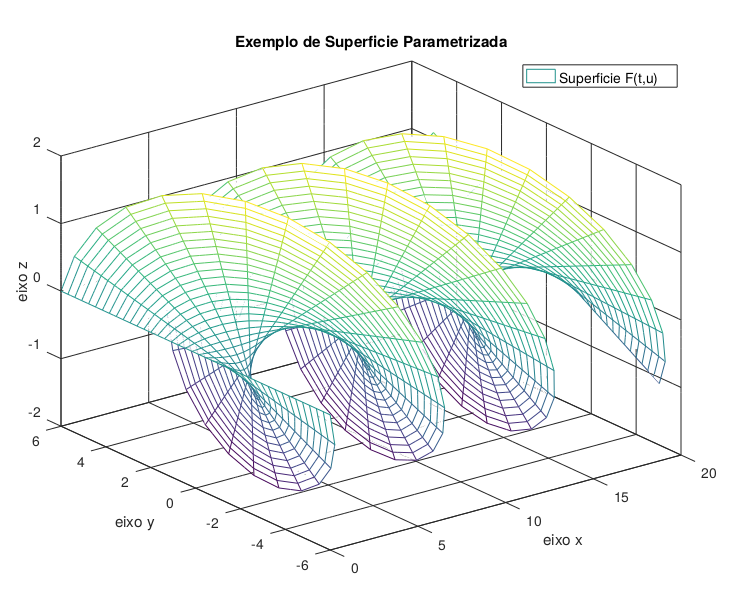
\includegraphics[angle=0,scale=0.4]{imagens/cap2/pespmesh.png} 
\caption{Superf�cie $F(t,u) = (f(t,u), g(t,u), h(t,u))$, $t=[0,10]$, $u=[-2,2]$, $f(t,u)=2\ t$, $g(t,u)=3\ u\ cos(t)$, $h(t,u)=u\ sen(t)$ nos pontos de {\it grid}.} 
\label{fig.pespmesh}
\end{center}
\end{figure}

\newpage
\newpage

\markboth{Variedades}{Variedades Definidas Implicitamente}
\subsection{Variedades Definidas Implicitamente}\label{var_impl}

Dada uma fun\c{c}\~ao de classe $C^r$, $F : \R^n \rightarrow \R^k$, $n \geq k$,  o conjunto dos pontos onde $F$ se anula $\mathcal{M} = F^{-1}(0) = \{ x \in \R^n  \; | \: F(x) = 0 \}$, \'e uma variedade definida implicitamente se para todo ponto em $\mathcal{M}$ a derivada de $F$ neste ponto tem posto m\'aximo. Neste caso a variedade $\mathcal{M}$ tem dimens\~ao $n-k$ (veja o Teorema \ref{teo_VI} da Se\c{c}\~ao \ref{var_dif}). 

Os casos mais comuns geralmente vistos nos cursos de c\'alculo s\~ao:
\begin{itemize}
 \item Para $n=2$ e $k=1$, $F^{-1}(0)$ \'e uma curva em $\R^2$;
 \item Para $n=3$ e $k=2$, $F^{-1}(0)$ \'e uma curva em $\R^3$;
 \item Para $n=3$ e $k=1$, $F^{-1}(0)$ \'e uma superf\'icie em $\R^3$.
\end{itemize}


\noindent {\bf Exemplo 1:} Seja $f:\R^2 \rightarrow \R$ dada por  $F(x,y)=3.5^{-\sqrt{x^2+y^2}} cos(y) sin(x/2)$. A variedade $\mathcal{M}$ � representada na figura \ref{fig.projecao}-(a) e foi gerada usando o c�digo \ref{supcurvanivel} feito em Matlab/Octave. A figura \ref{fig.projecao}-(b) foi gerada usando o c�digo \ref{supcurvanivelb} e mostra o gr�fico de $F(x,y)$ e sua proje��o.

\begin{Codigo}[htpb]
\noindent\rule{13cm}{1.pt}
 \begin{verbatim}
px = py = linspace (-3, 3, 50)';                    % dom�nio
[x, y] = meshgrid (px, py);                         % gerando a malha
z = 3.5.^(-1.*sqrt(x.^2+y.^2)).*cos(y).*sin(0.5*x); % superficie z=f(x,y)
contour(x,y,z,10)                                   % 10 curvas de n�vel
xlabel('eixo x')                                    % legenda no eixo x
ylabel('eixo y')                                    % legenda no eixo y
legend('Plano xy');                                 % legenda
\end{verbatim} 
\caption{C�digo utilizado para gerar a figura \ref{fig.projecao}-(a) } 
\noindent\rule{13cm}{1.pt}
\label{supcurvanivel}
\end{Codigo}

\begin{Codigo}[htpb]
\noindent\rule{13cm}{1.pt}
\begin{verbatim}
px = py = linspace (-3, 3, 50)';                  % dom�nio
[x, y] = meshgrid (px, py);                       % gerando a malha
z=3.5.^(-1.*sqrt(x.^2+y.^2)).*cos(y).*sin(0.5*x); % superficie z=f(x,y)
surfc(x,y,z)                                      % plotando o grafico 
                                                  % de F(x,y) e algumas 
                                                  % curvas de n�vel
xlabel('eixo x')                                  % legenda no eixo x
ylabel('eixo y')                                  % legenda no eixo y
zlabel ('F(x,y)')                                 % legenda no eixo z
title('Exemplo de Superficie');                   % t�tulo
legend('Superficie z=F(x,y)');                    % legenda                          
\end{verbatim}
\caption{C�digo utilizado para gerar a figura \ref{fig.projecao}-(b) } 
\noindent\rule{13cm}{1.pt}
\label{supcurvanivelb}
\end{Codigo}



\begin{figure}[htpb]
 \begin{tabular}{cc}
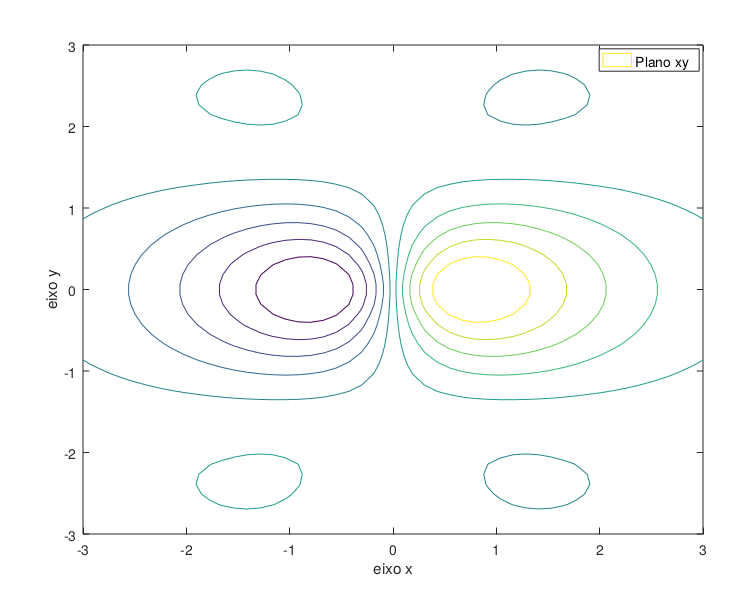
\includegraphics[angle=0,scale=0.3]{imagens/cap2/projxy.png} & 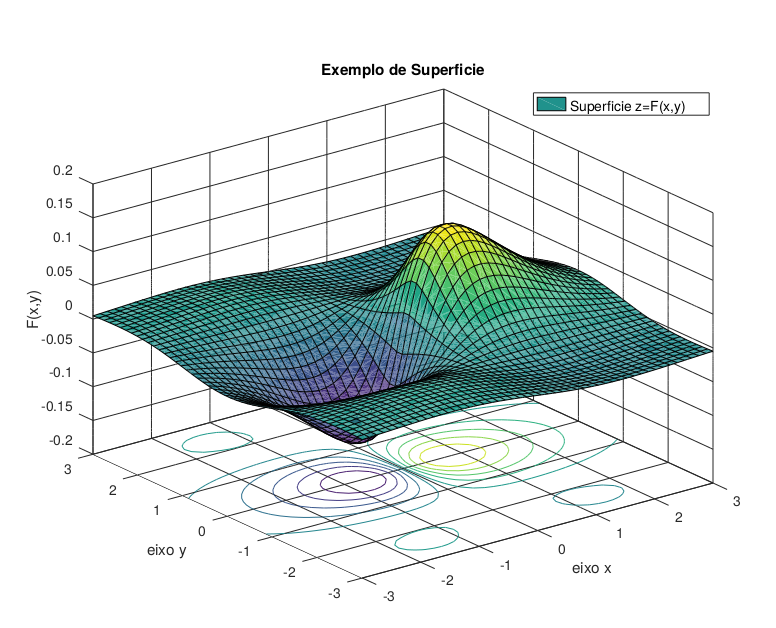
\includegraphics[angle=0,scale=0.4]{imagens/cap2/projecao.png} \\
(a) & (b) 
\end{tabular}
\caption{Superficie $F(x,y)=3.5^{-\sqrt{x^2+y^2}} cos(y) sin(x/2)$.}
\label{fig.projecao}
\end{figure}



\noindent {\bf Exemplo 2:} Seja $f:\R^3 \rightarrow \R$ dada por $f(x, y, z) = x^2 + y^2 + z^2$ . A esfera {$S^2$} de raio $r=2$ fica definida implicitamente pela equa��o $f(x,y,z) = 4$. A figura \ref{fig.esfera} mostra a Isosuperf�cie gerada pelo c�digo abaixo, feito em Matlab/Octave

\begin{Codigo}[htpb]
\noindent\rule{13cm}{1.pt}
\begin{verbatim}
[x,y,z] = meshgrid(-2:0.2:2,-2:0.2:2,-2:0.2:2); % gerando a malha
F = x.^2 + y.^2 + z.^2 -4.0 ;                   % esfera 
isosurface(x,y,z,F,0);                          % isosuperf�cie
axis equal;
xlabel('eixo x')                                % legenda no eixo x
ylabel('eixo y')                                % legenda no eixo y
zlabel('eixo z')                                % legenda no eixo z
legend('Esfera');                               % legenda
\end{verbatim}
\caption{C�digo utilizado para gerar a figura \ref{fig.esfera}} 
\noindent\rule{13cm}{1.pt}
\label{esfera}
\end{Codigo}


\begin{figure}[htpb]
\begin{center} 
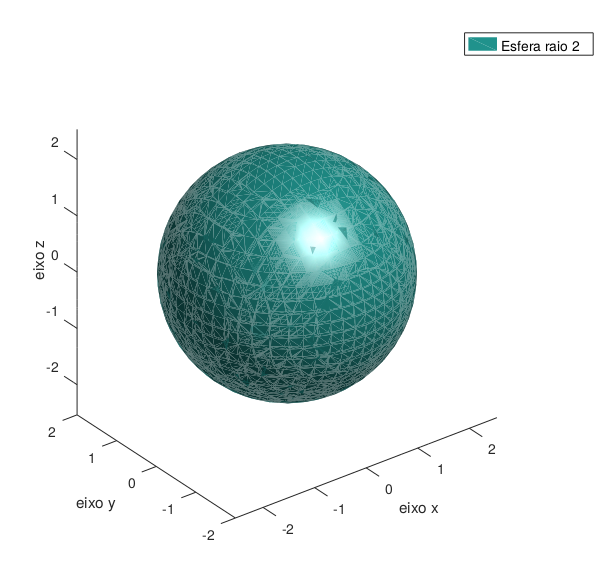
\includegraphics[angle=0,scale=0.5]{imagens/cap2/esfera_isosurf.png} 
\caption{Isosuperf�cie $F(x,y,z)=x^2+y^2+z^2-4.0$} 
\label{fig.esfera}
\end{center}
\end{figure}


\noindent {\bf Exemplo 3:} Seja $F:\R^3 \rightarrow \R^2$ dada por $F(x,y,z) = (f_1(x,y,z),f_2(x,y,z))$, onde $f_1(x,y,z)= x^2 + y^2 + z^2 - 1$ e $f_2(x,y,z)= 2x^2 + 2y^2 - 1$.
O conjunto $f_1^{-1}(0)$ � a esfera {$S^2$} de raio $r=1$ e o conjunto $f_2^{-1}(0)$ � um cilindro. 
A figura \ref{fig.isosurfr3r2}-(a) mostra as isosuperf�cies gerada pelo c�digo, feito em Matlab/Octave. Neste caso, $F^{-1}({\bf 0})=f_1^{-1}(0)\bigcap f_2^{-1}(0)$ s�o os c�rculos nos planos $z=\sqrt{2}$ e $z=-\sqrt{2}$ mostrados na figura \ref{fig.isosurfr3r2}-(b). 

\begin{Codigo}[htpb]
\noindent\rule{13cm}{1.pt}
\begin{verbatim}
[x,y,z] = meshgrid(-2:0.2:2,-2:0.2:2,-2:0.2:2); % gerando a malha
f1 = x.^2 + y.^2 + z.^2 -1.0 ;                  % esfera
f2 =2.0.*x.^2 + 2.0.*y.^2 -1.0 ;                % cilindro                        
isosurface(x,y,z,f1,0.1);                       % isosuperf�cie
isosurface(x,y,z,f2,0);                         % isosuperf�cie
camlight;
lighting gouraud;
axis equal;
xlabel('eixo x')                                % legenda no eixo x
ylabel('eixo y')                                % legenda no eixo y
zlabel('eixo z')                                % legenda no eixo z
\end{verbatim}
\caption{C�digo utilizado para gerar a figura \ref{fig.isosurfr3r2}} 
\noindent\rule{13cm}{1.pt}
\label{isosurfr3r2}
\end{Codigo}


\begin{figure}[htpb]
 \begin{tabular}{cc}
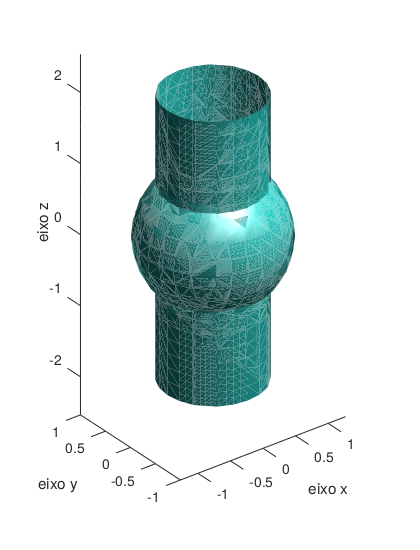
\includegraphics[angle=0,scale=0.46]{imagens/cap2/isosurfr3r2.png} & 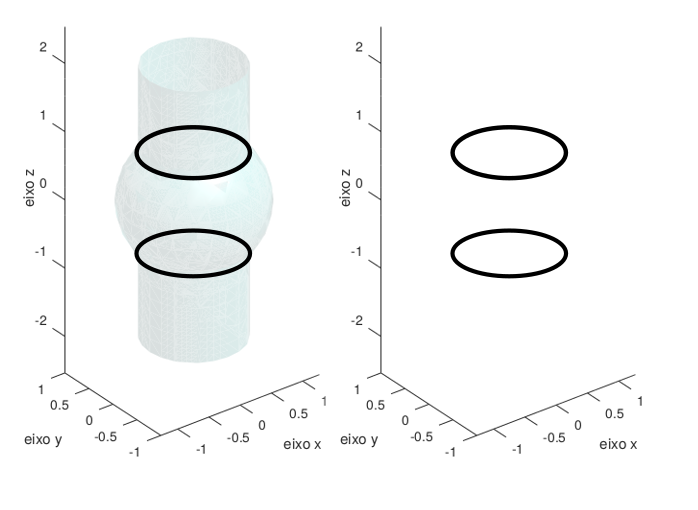
\includegraphics[angle=0,scale=0.35]{imagens/cap2/isosurfr3r2_2.png} \\
(a) & (b) 
\end{tabular}
\caption{Isosuperf�cie $F(x,y,z)=(f_1(x,y,z),f_2(x,y,z))$} 
\label{fig.isosurfr3r2}
\end{figure}

\newpage

\noindent {\bf Exemplo 4:} Seja $F:\R^3 \rightarrow \R$ dada por $F(x,y,z) = x^2 + y^2 - z^2$. 
A isosuperf�cie 0 da fun��o $F(x,y,z)$ � um cone, que � uma variedade exceto pela origem que � uma singularidade. 
Enquanto as isosuperf�cies 0 das fun��es  $G_1(x,y,z) = x^2 + y^2 - z^2 - 1.0$ e $G_2(x,y,z)=x^2 + y^2 - z^2 + 1.0$ s�o variedades definidas implicitamente. 
As figuras \ref{fig.cone}, \ref{fig.hipumafolha} e \ref{fig.hipduasfolhas} representam as isosuperf�cies 0, geradas em Matlab/Octave, do cone, de um hiperboloide de uma folha e um hiperboloide de duas folhas respectivamente.

\begin{Codigo}[htpb]
\noindent\rule{13cm}{1.pt}
\begin{verbatim}
[x,y,z] = meshgrid(-2:0.2:2,-2:0.2:2,-2:0.2:2); % gerando a malha
F = x.^2 + y.^2 - z.^2;                         % cone
isosurface(x,y,z,F,0);                          % isosuperf�cie
axis equal;
xlabel('eixo x')                                % legenda no eixo x
ylabel('eixo y')                                % legenda no eixo y
zlabel('eixo z')                                % legenda no eixo z
legend('Par cones');                            % legenda 
\end{verbatim}
\caption{C�digo utilizado para gerar a figura \ref{fig.cone}} 
\noindent\rule{13cm}{1.pt}
\label{supcurvanivelb}
\end{Codigo}

\begin{figure}[htpb]
\begin{center} 
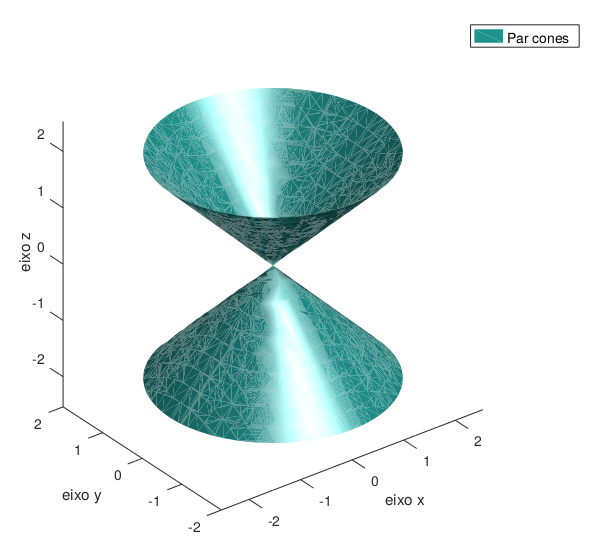
\includegraphics[angle=0,scale=0.7]{imagens/cap2/parcones.png} 
\caption{Isosuperf�cie $F(x,y,z)=x^2+y^2-z^2$} 
\label{fig.cone}
\end{center}
\end{figure}


\begin{Codigo}[htpb]
\noindent\rule{13cm}{1.pt}
\begin{verbatim}
[x,y,z] = meshgrid(-2:0.2:2,-2:0.2:2,-2:0.2:2); % gerando a malha
G_1 = x.^2 + y.^2 - z.^2 - 1.0;                 % hiperbol�ide
isosurface(x,y,z,G_1,0);                        % isosuperf�cie
axis equal;
xlabel('eixo x')                                % legenda no eixo x
ylabel('eixo y')                                % legenda no eixo y
zlabel('eixo z')                                % legenda no eixo z
legend('Hiperboloide uma folha ');              % legenda 
\end{verbatim}
\caption{C�digo utilizado para gerar a figura \ref{fig.hipumafolha}} 
\noindent\rule{13cm}{1.pt}
\label{supcurvanivelb}
\end{Codigo}

\begin{figure}[htpb]
\begin{center} 
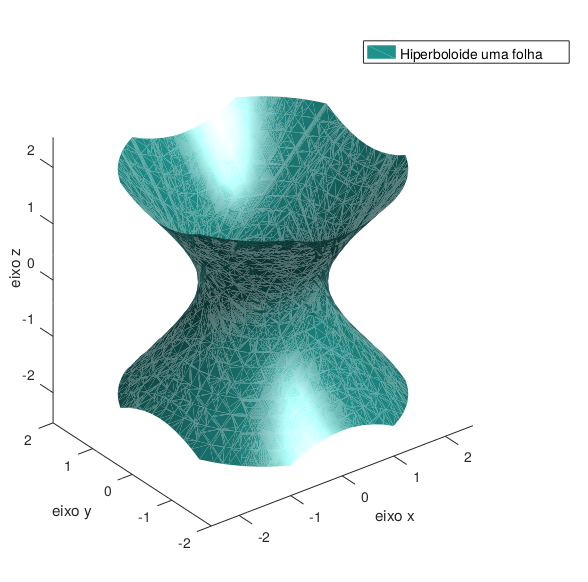
\includegraphics[angle=0,scale=0.7]{imagens/cap2/hipumafolha.png} 
\caption{Isosuperf�cie $G_1(x,y,z)=x^2+y^2-z^2-1.0$} 
\label{fig.hipumafolha}
\end{center}
\end{figure}



\begin{Codigo}[htpb]
\noindent\rule{13cm}{1.pt}
\begin{verbatim}
[x,y,z] = meshgrid(-2:0.2:2,-2:0.2:2,-2:0.2:2); % gerando a malha
G_2 = x.^2 + y.^2 - z.^2 + 1.0;                 % hiperbol�ide
isosurface(x,y,z,G_2,0);                        % isosuperf�cie
axis equal;
xlabel('eixo x')                                % legenda no eixo x
ylabel('eixo y')                                % legenda no eixo y
zlabel('eixo z')                                % legenda no eixo z
legend('Hiperboloide duas folhas ');            % legenda 
\end{verbatim}
\caption{C�digo utilizado para gerar a figura \ref{fig.hipduasfolhas}} 
\noindent\rule{13cm}{1.pt}
\label{supcurvanivelb}
\end{Codigo}

\begin{figure}[htpb]
\begin{center} 
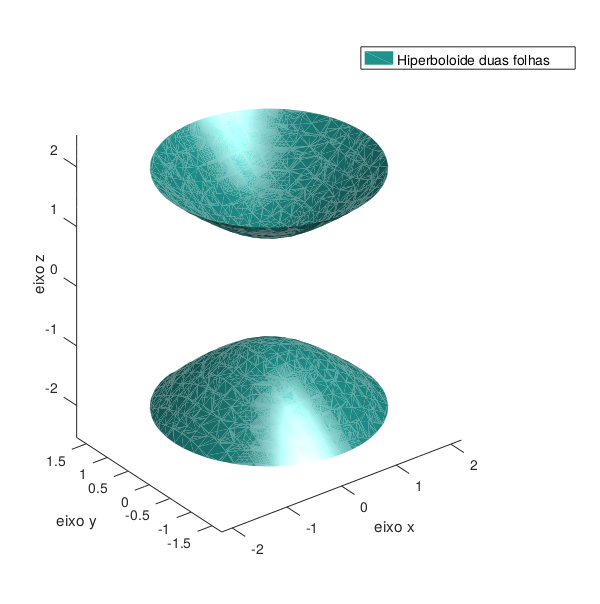
\includegraphics[angle=0,scale=0.7]{imagens/cap2/hipduasfolhas.png} 
\caption{Isosuperf�cie $G_2(x,y,z)=x^2+y^2-z^2+1.0$} 
\label{fig.hipduasfolhas}
\end{center}
\end{figure}





% Para se ter uma ideia melhor de uma aproxima\c{c}\~ao de variedade, a Figura~\ref{fig.toro3d} mostra um toro tridimensional, $S^2 \times S^1$ ($S^1$ \'e uma esfera unidimensional e $S^2$ \'e uma esfera bidimensional). 
% Neste exemplo, $F : \R^5 \rightarrow \R^2$ \'e definida por
% $$ 
% \left\{
% \begin{array}{llll}
% F_1(x_1,x_2,x_3,x_4,x_5) & = x_1^2 + x_2^2 + x_3^2 & - & 1 \\
% F_2(x_1,x_2,x_3,x_4,x_5) & = x_4^2 + x_5^2         & - & \frac{1}{4}
% \end{array} 
% \right.
% $$ 

% \begin{figure}[htpb]
% \begin{center} 
% \includegraphics[angle=0,scale=0.4]{imagens/S2xS1_CS.png} 
% \caption{Proje\c{c}\~ao da aproxima\c{c}\~ao de um toro $S^2 \times S^1$ definido em $\R^5$.} 
% \label{fig.toro3d}
% \end{center}
% \end{figure}

\pagebreak

\markboth{Variedades}{Exerc�cios}
\section{Exerc�cios}\label{exerc}

\begin{enumerate}

\item Gere um c�digo em Matlab/Octave  que gere uma superf�cie em $\R^3$ como gr�fico de fun��o utilizando os comandos {\it surf} e {\it mesh}. 

\item Escreva as equa��es de um c�rculo parametrizado em $\R^2$, utilize coordenadas polares.

\item Escreva as equa��es de uma elipse parametrizada em $\R^2$.

\item Gere um c�digo em Matlab/Octave que gere uma curva fechada parametrizada da sua escolha em $\R^2$.

\item Gere um c�digo em Matlab/Octave que gere uma curva fechada parametrizada da sua escolha em $\R^3$.

\item Gere um c�digo em Matlab/Octave que gere uma superf�cie parametrizada da sua escolha em $\R^3$.

\item Escreva as equa��es de um cilindro parametrizado em $\R^3$, utilize coordenadas cil�ndricas.

\item Gere um c�digo em Matlab/Octave que gere um cilindro parametrizado em $\R^3$, utilizando coordenadas cil�ndricas.

\item Escreva as equa��es de uma esfera parametrizada em $\R^3$, utilize coordenadas esf�ricas.

\item Escreva as equa��es de um elipsoide parametrizado em $\R^3$.

\item Gere um c�digo em Matlab/Octave que gere uma esfera parametrizada em $\R^3$, utilizando coordenadas esf�ricas.

\item Gere um c�digo em Matlab/Octave que gere um elipsoide definido implicitamente em $\R^3$.

\item Gere um c�digo em Matlab/Octave que gere um toro definido implicitamente em $\R^3$.

\end{enumerate}
 % Variedeades
\chapter{Estruturas de Dados para Variedades Lineares por Partes}\label{cap_est_dados}

\thispagestyle{empty}

\markboth{Estruturas de Dados para Variedades Lineares por Partes}{Estruturas de Dados Expl�citas}
\section{Estruturas de Dados Expl�citas}\label{ed_ede}

\markboth{Estruturas de Dados para Variedades Lineares por Partes}{Estruturas de Dados Impl�citas}
\section{Estruturas de Dados Impl�citas}\label{ed_edi}

 % Estruturas de dados para superf�cies 
\chapter{Modelagem Utilizando Operadores Diferenciais}\label{cap_mod_od}

\thispagestyle{empty}


\markboth{Modelagem Utilizando Operadores Diferenciais}{Operador de Laplace-Beltrami}
\section{Operador de Laplace-Beltrami}\label{proc_ilb}


\markboth{Modelagem Utilizando Operadores Diferenciais}{Reconstru��o de Superf�cies Lineares por Partes}
\section{Reconstru��o de Superf�cies Lineares por Partes}\label{proc_recsup}
 % Reconstru��o de superf�cies
\chapter{Variedades Definidas Implicitamente}\label{cap_var_imp}

\thispagestyle{empty}

Para maior aprofundamento no tema apresentado nesta e nas pr\'oximas se��es, \'e sugerida a leitura da tese~\cite{Cas92}, do livro~\cite{AlGe90}, do artigo~\cite{Cas06} e do curso no proceedings~\cite{Eaves76}. 

\markboth{Aproxima\c{c}\~oes de Fun\c{c}\~oes Impl\'{\i}citas}{Interpola\c{c}\~ao Linear Simplicial}
\section{Interpola\c{c}\~ao Linear Simplicial}\label{vi_ilp}


\begin{defi} $($Aproxima��o Simplicial$)$
Seja $F : S \subset  \R^{n} \rightarrow \R^{k}$ uma aplica\c c\~ao e $T$ uma triangula\c c\~ao de $S$.
Se $\sigma = [v_{0},\ldots,v_{n}] \in T$, tem-se para cada $v \in
\sigma$ uma \'unica $(n+1)$-upla $\lambda = (\lambda_{0}, \ldots,\lambda_{n})$ 
tal que $\sum_{i=0}^{n} \lambda_{i} v_{i} = v$, 
$\sum_{i=0}^{n} \lambda_{i} = 1$ e $\lambda_{i} \geq 0$, $i = 0,\ldots,n$.
Define-se $F_{\sigma} : \sigma \rightarrow \R^{k}$ onde
$F_{\sigma}(v) = F_{\sigma}(\sum_{i=0}^{n} \lambda_{i} v_{i}) = \sum_{i=0}^{n} \lambda_{i} F(v_{i})$.
\end{defi}

Observe que $F_{\sigma}$ \'e uma aplica\c c\~ao afim e que
$F_{\sigma}(v_{i}) = F(v_{i})$, $i = 0, \ldots, n$, isto \'e,
$F_{\sigma}$ \'e uma interpola\c c\~ao linear de $F$ nos v\'ertices de $\sigma$.

\begin{defi} $($Aproxima��o Linear por Partes$)$
Define-se uma aproxima\c c\~ao linear por partes para $F$ sendo, 
$F_{T} : S \subset  \R^{n} \rightarrow  \R^{k}$ onde 
$F_{T}(v) = F_{\sigma}(v)$ para $v \in \sigma \in T$.
\end{defi}

Portanto, $F_{T}$ \'e uma interpola\c c\~ao de $F$ para os
v\'ertices de $T$ (nos simplexos de dimens\~ao zero de $T$) e que \'e afim em
cada simplexo de dimens\~ao $n$ de $T$.

\begin{teore} \label{teo_AG}
Sejam $S \subset \R^{n}$ aberto,  $F : S \rightarrow \R^{k}$  uma
aplica\c c\~ao de classe $C^{2}$ com $\parallel D^{2}F(x) \parallel
\leq \alpha$ para todo $x \in S$ e $\sigma = [v_{0}, \ldots, v_{n}]$
um simplexo de uma triangula\c c\~ao robusta $T$ de $S$ $(\theta(T) > 0)$, ent\~ao 
\begin{enumerate}
\item $\parallel F(v) - F_{T}(v) \parallel \leq \alpha \rho^{2}(T)/2$ 
para todo $v \in S$ e 
\item $\parallel DF(v) - DF_{T}(v) \parallel \leq \alpha \rho(T)/\theta(T)$ para 
todo $v$ no interior de simplexos de dimens\~ao $n$ de $T$.
\end{enumerate}
\end{teore}

Embora $DF_{\sigma}(v)$ esteja bem definida para todo simplexo
$\sigma$ de dimens\~ao $n$, se $\tau$ \'e uma face comum de dois
simplexos $\sigma_{1}$ e $\sigma_{2}$ de  dimens\~ao $n$ e $v \in
\tau, DF_{\sigma_{1}}(v)$ e $DF_{\sigma_{2}}(v)$ podem ser distintas
e, portanto, $DF_{T}(v)$ n\~ao est\'a bem definida.



%\markboth{Aproxima\c{c}\~oes de Fun\c{c}\~oes Impl\'icitas}{Esquema de Diferen\c{c}as Simplicial}
%\section{Esquema de Diferen\c{c}as Simplicial}\label{vi_eds}
%
%Esta se��o e a pr�xima s�o importante para mostrar o funcionamento das aproxima��es de variedades impl�citas e suas limita��es.
%
%Seja $F : S \subset  \R^{n} \rightarrow \R^{k}$ uma 
%aplica\c c\~ao de classe $C^{2}$ e $T$ uma triangula\c c\~ao de $S$.
%
%Seja $\sigma = [v_{0}, \ldots, v_{n}] \in T$. Como $\sigma$ \'e um
%simplexo de dimens\~ao $n$, os vetores 
%$\{ v_{1}-v_{0}$, $v_{2}-v_{0},\ldots,v_{n}-v_{0}\}$ s\~ao linearmente 
%independentes; logo, fazendo \\ $\delta_{i} = \parallel v_{i}-v_{0} \parallel$ e 
%$\omega_{i} = (v_{i}-v_{0})/\delta_{i}$, $i = 1,\ldots,n$, temos que a
%matriz cujas colunas s\~ao os vetores $\{\omega_{1},\ldots,\omega_{n}\}$ \'e 
%invert\'{\i}vel. 
%
%Para $v \in \sigma$, seja $\lambda$, tal que $\sum_{i=0}^{n} \lambda_{i} v_{i} 
%= v$, $\sum_{i=0}^{n} \lambda_{i} = 1$ e $\lambda_{i} \geq 0$, 
%$i = 0,\ldots,n$. Ent\~ao, pode-se escrever 
%$$
%\begin{array}{l}
  %v - v_{0} = \\
 %\sum^{n}_{i=0} \lambda_{i} v_{i} - v_{0} \sum^{n}_{i=0} \lambda_{i} = \\
 %\sum^{n}_{i=1} \lambda_{i} (v_{i} - v_{0}) = \\
 %\sum^{n}_{i=1} \lambda_{i} \delta_{i} \omega_{i} = \\
 %\left( \omega_{1} \cdots \omega_{n} \right)
  %\left(  
  %\begin{array}{c}
  %\lambda_{1} \delta_{1} \\
  %\vdots \\
  %\lambda_{n} \delta_{n} 
  %\end{array}
  %\right)
%\end{array}
%$$
%ou
%$$ 
%\left( 
%\begin{array}{c}
%\lambda_{1} \delta_{1} \\
%\vdots \\
%\lambda_{n} \delta_{n}
%\end{array}
%\right) 
 %= 
%\left( \omega_{1} \cdots \omega_{n} \right)^{-1} 
%\left( v - v_{0} \right). 
%$$
%
%Agora
%$$
%\begin{array}{l}
  %F_{T}(v) - F(v_{0}) = \\
 %F_{\sigma}(v) - F(v_{0}) = \\
 %\sum^{n}_{i=0} \lambda_{i} F(v_{i}) - F(v_{0}) \sum^{n}_{i=0} \lambda_{i} =\\
 %\sum^{n}_{i=1} \lambda_{i} (F(v_{i}) - F(v_{0})) = \\
 %\sum^{n}_{i=1} \lambda_{i} \delta_{i} (F(v_{i})- F(v_{0}))/\delta_{i}  
%\end{array}
%$$
%ou
%$$
%\begin{array}{l}
  %F_{T}(v) - F(v_{0}) = \\
 %\left( \frac{F(v_{1})-F(v_{0})}{\delta_{1}} \cdots 
         %\frac{F(v_{n})-F(v_{0})}{\delta_{n}} \right) 
  %\left(
  %\begin{array}{c}
  %\lambda_{1} \delta_{1} \\
  %\vdots \\
  %\lambda_{n} \delta_{n}
  %\end{array}
  %\right) = \\
 %\left( \frac{F(v_{1})-F(v_{0})}{\delta_{1}} \cdots 
         %\frac{F(v_{n})-F(v_{0})}{\delta_{n}} \right) 
  %\left( \omega_{1} \cdots \omega_{n} \right)^{-1} 
  %\left( v-v_{0} \right).
%\end{array}
%$$
%
%Da\'{\i}, como $\omega_{i} = (v_{i}-v_{0})/\delta_{i}$, tem-se
%$v_{i} = v_{0}+\delta_{i}\omega_{i}$, $i= 1,\ldots,n$, e portanto
%{\scriptsize
%$$
%F_{T}(v) - F(v_{0}) = 
%\left(
%\frac{F(v_{0}+\delta_{1}\omega_{1})-F(v_{0})}{\delta_{1}}
%\cdots 
%\frac{F(v_{0}+\delta_{n}\omega_{n})-F(v_{0})}{\delta_{n}}
%\right)
%\left(
%\omega_{1} \cdots \omega_{n}
%\right)^{-1}  
%\left(
%v-v_{0} 
%\right). 
%$$
%}
%
%Observe que as colunas da matriz
%$$
%\left(
%\frac{F(v_{0}+\delta_{1}\omega_{1})-F(v_{0})}{\delta_{1}}
%\cdots  
%\frac{F(v_{0}+\delta_{n}\omega_{n})-F(v_{0})}{\delta_{n}}
%\right)
%$$
%s\~ao aproxima\c c\~oes para as derivadas direcionais de
%$F$ nas dire\c c\~oes $\omega_{1},\ldots,\omega_{n}$, em torno do ponto
%$v_{0}$; portanto este \'e um esquema de diferen\c cas que 
%chamaremos de esquema de diferen\c cas simplicial. 
%
%Assim, se $\delta_{i} \rightarrow 0$ para $i= 1, \ldots, n$ com
%uma certa proporcionalidade, isto \'e, se o di\^ametro de $\sigma$
%tende a zero mantendo a robustez limitada para que os vetores 
%$\omega_{1},\ldots,\omega_{n}$ continuem sendo linearmente independentes, 
%ent\~ao $F_{\sigma}$ \'e uma apro\-xima\c c\~ao para os dois primeiros 
%termos da s\'erie de Taylor de $F$, em torno do ponto $v_{0}$.
%Outra observa\c c\~ao \'e que a mesma an\'alise pode ser feita para
%qualquer outro v\'ertice de $\sigma$; portanto, o esquema descrito anteriormente
%n\~ao depende apenas do ponto $v_{0}$ e sim do simplexo $\sigma$.
%

\markboth{Aproxima\c{c}\~oes de Fun\c{c}\~oes Impl\'icitas}{Resultados sobre Aproxima��es Simpliciais}
\section{Resultados sobre Aproxima��es Simpliciais}\label{vi_ari}


Seja $F : U \rightarrow \R^{k}$ uma aplica\c c\~ao de classe $C^{p}$ no aberto $U \subset \R^{n}$, com $n > k$, $p > max\{ 1, n/k -1\}$ e tendo ${\bf 0} \in \R^{k}$ como valor regular. Considere a variedade de dimens\~ao $n-k$ e classe $C^{p}$, $\mathcal{M} = F^{-1}({\bf 0})$ e uma vizinhan\c ca tubular de $\mathcal{M}$, $V_\mathcal{M}$, tal como no Teorema \ref{teo_VT}.

Como desejamos uma aproxima\c c\~ao de $\mathcal{M}$ que possa ser representada computacionalmente, vamos restringir o dom\'{\i}nio de $F$ a um compacto $S \subset U$. Assim, existe $\alpha > 0$ tal que $\parallel D^{2} F(x)\parallel \leq \alpha$ para todo $x \in K$ e, portanto, se $T$ for uma triangula\c c\~ao robusta de $S$, fica valendo o Teorema \ref{teo_AG} para $F_{T}$.

Para estabelecermos algumas propriedades sobre a aproxima\c c\~ao $\mathcal{M}_{T} = F_{T}^{-1}({\bf 0})$ de $\mathcal{M}$, vamos observar algumas propriedades que $F$ e $T$ devem satisfazer. 

Seja $\sigma = [v_{0}, \ldots, v_{k}]$ um simplexo de dimens\~ao $k$ de $U$. Para que $F_{\sigma}(\sigma) = [F(v_{0}),\ldots,F(v_{k})]$ seja um simplexo de dimens\~ao $k$ em $\R^{k}$, basta que os de vetores $F(v_{1})-F(v_{0}),\ldots,F(v_{k})-F(v_{0})$ sejam linearmente independentes, pelo fato de $F_{\sigma}$ ser uma aplica\c c\~ao afim.
Neste caso, se $\tau$ \'e uma face de $\sigma$ de dimens\~ao $r \leq k$, teremos que $F_{\sigma}(\tau)$ \'e uma face de $F_{\sigma}(\sigma)$ de dimens\~ao $r$. 

Com rela\c c\~ao a este assunto temos o seguinte teorema:

\begin{teore} {\rm $($Veja~\cite{Fr91}$)$} \label{teo_Fr91_1}
Para quase todo simplexo $\sigma$ de dimens\~ao $r \leq k$ de $S \cap V_\mathcal{M}$, temos que $F_{\sigma}(\sigma)$ \'e um simplexo de dimens\~ao $r$ em $\R^{k}$.
\end{teore}


\begin{defi} 
Diremos que $v \in \sigma = [v_{0},\ldots,v_{n}] \in T$ \'e um ponto regular de $F_{T}$, se $DF_{\sigma}(v)$ for sobrejetora, ou de forma equivalente, que a matriz 
$$
\left( 
\begin{array}{ccc}
1 & \cdots & 1 \\
F(v_{0}) & \cdots & F(v_{n})
\end{array} 
\right)
$$
tenha posto $k+1$. 
Se $v$ n\~ao for um ponto regular de $F_{T}$, diremos que
\'e um ponto cr\'{\i}tico de $F_{T}$. 
Diremos que $c \in \R^{k}$ \'e valor regular de $F_{T}$ se todo $v \in F_{T}^{-1}(c)$ for ponto regular de $F_{T}$. 
Se $c$ n\~ao for valor regular de $F_{T}$, diremos que \'e valor cr\'{\i}tico de $F_{T}$.
\end{defi} 

\begin{teore} {\rm $($Veja~\cite{Eaves76}$)$} \label{teo_Ea76}
Seja $T$ uma triangula��o de $S$. Se $0 \in \R^{n}$ for valor regular de $F_{T}$, ent\~ao $\mathcal{M}_{T} = F_{T}^{-1}(0)$ \'e uma variedade linear por partes de dimens\~ao $n-k$.
\end{teore} 

Observe-se que o teorema \ref{teo_Ea76} n\~ao garante que $F_{T}^{-1}(0) \cap \sigma$ seja uma c\'elula de dimens\~ao $r$ se $\sigma$ for um simplexo de dimens\~ao $k+r$, $r = 1,\ldots,n-k$.  
Com rela\c c\~ao a esta observa\c c\~ao, temos o seguinte exemplo:
$ F : \R^{2} \rightarrow \R$ definida por $F(x,y) = x + 2y$ e 
$\sigma = [v_{0},v_{1},v_{2}]$ com $v_{0} = (0, 0), v_{1} = (1, 0)$ e 
$v_{2} = (0, 1)$. Como $F(v_{0}) = 0, F(v_{1}) = 1$ e $F(v_{2}) = 2$, temos
que $F_{\sigma}^{-1}(0) \cap \sigma = \{(0, 0)\}$, que \'e uma
c\'elula de dimens\~ao $0$.

Como $DF(x)$ tem posto $k$ para todo $x \in S \cap V_\mathcal{M}$, a inversa de Moore-Penrose para $DF(x)$, $DF(x)^{+} = DF(x)^{t} \cdot (DF(x) \cdot DF(x)^{t})^{-1}$ est\'a bem definida. 
Como $S \cap V_\mathcal{M}$ \'e um conjunto compacto, existe $\mu > 0$, tal que $\parallel DF(x)^{+} \parallel \leq \mu$ para todo $x \in S \cap V_\mathcal{M}$. 

\begin{teore} {\rm $($Veja~\cite{Fr91}$)$} \label{teo_Fr91_2}
Para quase todo simplexo $\sigma$ de dimens\~ao $k$ de $S \cap V_\mathcal{M}$ com $\alpha \mu \rho(\sigma)/\theta(\sigma) < 1$, cujo interior intercepta $\mathcal{M}$, temos que o interior de $\sigma$ intercepta $\mathcal{M}_{\sigma}$. 
\end{teore} 

Como $S$ \'e compacto, para quase toda triangula\c c\~ao $T$ de $S$, seus simplexos de dimens\~ao maior ou igual a $k$ t\^em interior transversal a $\mathcal{M}$. 
Da\'{\i}, segue o corol\'ario do teorema \ref{teo_Fr91_2}.

\begin{corol} {\rm $($Veja~\cite{Fr91}$)$} \label{cor_Fr91}
Para quase toda triangula\c c\~ao robusta $T$ de $S$ com di\^ametro suficientemente pequeno, temos que todo simplexo de dimens\~ao maior ou igual a $k$ tem interior transversal a $\mathcal{M}$ e $\mathcal{M}_{T}$, e se intercepta $\mathcal{M}$, ent\~ao tamb\'em intercepta $\mathcal{M}_{T}$. 
\end{corol} 
 
O corol\'ario \ref{cor_Fr91} nos d\'a duas propriedades muito importantes: 
para quase toda triangula\c c\~ao $T$ de $S$ com di\^ametro suficientemente
pequeno, temos 
\begin{itemize}
\item se $\sigma$ for um simplexo de dimens\~ao $k$ de $T$ e $x \in \sigma \cap \mathcal{M}$, existe $v \in \sigma \cap \mathcal{M}_{T}$ e consequentemente $d(x, v) = \parallel x-v \parallel \leq \rho(\sigma) \leq \rho(T)$; 
\item se $\sigma$ for um simplexo de dimens\~ao $k+r$ de $T$ com $0 \leq r \leq n-k$, temos que se $F_{T}^{-1}(0) \cap \sigma \neq \emptyset$, ent\~ao $F_{T}^{-1}(0) \cap \sigma$ \'e uma c\'elula convexa afim de dimens\~ao $r$. 
\end{itemize}

A segunda propriedade ser\'a muito importante para representa\c c\~ao computacional das c\'elulas de $\mathcal{M}_{T}$. 
Tamb\'em com rela\c c\~ao \`a aproxima\c c\~ao entre $\mathcal{M}$ e $\mathcal{M}_{T}$, temos os seguintes teoremas:

\begin{teore} {\rm $($Veja~\cite{GaZa80}$)$} \label{teo_GaZa80}
Dado $\epsilon > 0$, existe uma triangula\c c\~ao $T$ de $S$ tal que, se $v \in \mathcal{M}_{T} = F_{T}^{-1}(0)$, ent\~ao $d(v,\mathcal{M}) = inf \{\parallel u-v\parallel ; u \in \mathcal{M} \} < \epsilon$. 
\end{teore} 

\begin{teore} {\rm $($Veja~\cite{AlGe80}$)$} \label{teo_AG80}
Sejam $x \in \mathcal{M}$ e $y \in \mathcal{M}_{T}$. 
Se $\parallel x-y \parallel \leq 1/(\alpha \mu)$, ent\~ao $\parallel x-y \parallel \leq \alpha \mu \rho^{2}(T)$.
\end{teore} 


 % Variedades Impl�citas
\chapter{Curvas e Sperf�cies NURBS}\label{cap_NURBS}

\thispagestyle{empty}

\markboth{Curvas e Sperf�cies NURBS}{Curvas e Superf�cies de Bezier}
\section{Curvas e Superf�cies de Bezier}\label{N_B}

\markboth{Curvas e Sperf�cies NURBS}{Curvas e Superf�cies B-Splines}
\section{Curvas e Superf�cies B-Splines}\label{N_BS}

\markboth{Curvas e Sperf�cies NURBS}{Curvas e Superf�cies Racional B-Splines}
\section{Curvas e Superf�cies Racional B-Splines}\label{N_RBS}

\markboth{Curvas e Sperf�cies NURBS}{Curvas e Superf�cies NURBS}
\section{Curvas e Superf�cies NURBS}\label{N_NURBS}

 % NURBS
\chapter{Caracter�sticas Robustas}\label{cap_car_rob}

\thispagestyle{empty}


\markboth{Caracter�sticas Robustas}{Conceitos B�sicos de Geometria Diferencial}
\section{Conceitos B�sicos de Geometria Diferencial}\label{cr_gd}

\markboth{Caracter�sticas Robustas}{Caracter�sticas Robustas}
\section{Carcter�sticas Robustas}\label{cr_gd}

 % Curvas robustas
\bibliographystyle{abnt-alf}
\bibliography{references}

\printindex

\end{document}
